% Seminarul 12: Modele de scoring
% Statistica piețelor financiare -- Program de licență, Academia de Studii Economice din București
% GENERAT de latex/build_seminar12.py -- modificați generatorul, nu acest fișier.
% Implicit versiunea pentru studenți; versiunea profesorului este wrapper-ul *_solutions.tex.
\makeatletter\@ifundefined{ifsolutions}{\expandafter\newif\csname ifsolutions\endcsname}{}\makeatother

\newcommand{\coursename}{Statistica piețelor financiare}
\def\sfmlang{ro}
% Preambul comun SFM -- Statistica piețelor financiare / Statistics of Financial Markets (Beamer, 16:9)
% Același design ca MFM. Înainte de % Preambul comun SFM -- Statistica piețelor financiare / Statistics of Financial Markets (Beamer, 16:9)
% Același design ca MFM. Înainte de % Preambul comun SFM -- Statistica piețelor financiare / Statistics of Financial Markets (Beamer, 16:9)
% Același design ca MFM. Înainte de \input{../../latex/preamble} se definește
%   \newcommand{\coursename}{Statistics of Financial Markets}      (EN)
%   \newcommand{\coursename}{Statistica piețelor financiare}       (RO)  și  \def\sfmlang{ro}
% Fișierele .tex se află în EN/Courses, EN/Seminars, RO/Cursuri, RO/Seminarii (două niveluri sub rădăcină).
% Deck-urile sînt generate de latex/build_chapterN.py / build_seminarN.py (vezi latex/sfm_build.py).

\documentclass[9pt, aspectratio=169, t]{beamer}
\providecommand{\coursename}{Statistics of Financial Markets}

% Ensure content fits on slides
\setbeamersize{text margin left=8mm, text margin right=8mm}

%=============================================================================
% THEME AND STYLE CONFIGURATION
%=============================================================================
\usetheme{default}
% Using default theme for clean header/footer control

% Color Palette (matching Redispatch PDF)
\definecolor{MainBlue}{RGB}{26, 58, 110}
\definecolor{AccentBlue}{RGB}{26, 58, 110}
\definecolor{IDAred}{RGB}{205, 0, 0}
\definecolor{DarkGray}{RGB}{51, 51, 51}
\definecolor{MediumGray}{RGB}{128, 128, 128}
\definecolor{LightGray}{RGB}{248, 248, 248}
\definecolor{VeryLightGray}{RGB}{235, 235, 235}
\definecolor{KeynoteGray}{RGB}{218, 218, 218}
\definecolor{SectionGray}{RGB}{120, 120, 120}
\definecolor{FooterGray}{RGB}{100, 100, 100}
\definecolor{Crimson}{RGB}{220, 53, 69}
\definecolor{Forest}{RGB}{46, 125, 50}
\definecolor{Amber}{RGB}{181, 133, 63}
\definecolor{Orange}{RGB}{230, 126, 34}
\definecolor{Purple}{RGB}{142, 68, 173}

% Gradient background (exact Keynote 315° gradient: white to RGB 218,218,218)
\setbeamertemplate{background}{%
    \begin{tikzpicture}[remember picture, overlay]
        \shade[shading=axis, shading angle=315,
        top color=white, bottom color=KeynoteGray]
        (current page.south west) rectangle (current page.north east);
    \end{tikzpicture}%
}
% Fallback solid color for compatibility
\setbeamercolor{background canvas}{bg=}

\setbeamercolor{palette primary}{bg=MainBlue, fg=white}
\setbeamercolor{palette secondary}{bg=MainBlue!85, fg=white}
\setbeamercolor{palette tertiary}{bg=MainBlue!70, fg=white}
\setbeamercolor{structure}{fg=MainBlue}
\setbeamercolor{title}{fg=IDAred}
\setbeamercolor{frametitle}{fg=IDAred, bg=}
\setbeamercolor{block title}{bg=MainBlue, fg=white}
\setbeamercolor{block body}{bg=VeryLightGray, fg=DarkGray}
\setbeamercolor{block title alerted}{bg=Crimson, fg=white}
\setbeamercolor{block body alerted}{bg=Crimson!8, fg=DarkGray}
\setbeamercolor{block title example}{bg=Forest, fg=white}
\setbeamercolor{block body example}{bg=Forest!8, fg=DarkGray}
\setbeamercolor{item}{fg=MainBlue}

% Footer colors (override Madrid theme blue)
\setbeamercolor{author in head/foot}{fg=FooterGray, bg=}
\setbeamercolor{title in head/foot}{fg=FooterGray, bg=}
\setbeamercolor{date in head/foot}{fg=FooterGray, bg=}
\setbeamercolor{section in head/foot}{fg=FooterGray, bg=}
\setbeamercolor{subsection in head/foot}{fg=FooterGray, bg=}

% Bullet styles (apply everywhere including blocks)
\setbeamertemplate{itemize item}{\color{MainBlue}$\boxdot$}
\setbeamertemplate{itemize subitem}{\color{MainBlue}$\blacktriangleright$}
\setbeamertemplate{itemize subsubitem}{\color{MainBlue}\tiny$\bullet$}
\setbeamertemplate{itemize/enumerate body begin}{\normalsize}
\setbeamertemplate{itemize/enumerate subbody begin}{\normalsize}

% Item spacing - compact style
\setlength{\leftmargini}{10pt}       % Level 1: minimal indent
\setlength{\leftmarginii}{10pt}      % Level 2: minimal additional indent
% Compact list spacing (zero extra space before/after lists in blocks)
\makeatletter
\def\@listi{\leftmargin\leftmargini \topsep 0pt \parsep 0pt \itemsep 0pt}
\def\@listii{\leftmargin\leftmarginii \topsep 0pt \parsep 0pt \itemsep 0pt}
\makeatother

\setbeamertemplate{navigation symbols}{}

%=============================================================================
% CUSTOM HEADLINE
%=============================================================================
\setbeamertemplate{headline}{%
    \vskip10pt%
    \hbox to \paperwidth{%
        \hskip0.5cm%
        {\small\color{FooterGray}\renewcommand{\hyperlink}[2]{##2}\insertsectionhead}%
        \hfill%
        \textcolor{FooterGray}{\small\insertframenumber}%
        \hskip0.5cm%
    }%
    \vskip4pt%
    {\color{FooterGray}\hrule height 0.4pt}%
}

%=============================================================================
% CUSTOM FOOTER
%=============================================================================
\usepackage{fontawesome5}

\setbeamertemplate{footline}{%
    {\color{FooterGray}\hrule height 0.4pt}%
    \vskip4pt%
    \hbox to \paperwidth{%
        \hskip0.5cm%
        \textcolor{FooterGray}{\small\coursename}%
        \hfill%
        \raisebox{-0.1em}{%
            \begin{tikzpicture}[x=0.08em, y=0.08em, line width=0.4pt]
                \draw[FooterGray] (0,3) -- (1,4) -- (2,3.5) -- (3,5) -- (4,4) -- (5,6) -- (6,5.5) -- (7,4) -- (8,5) -- (9,7) -- (10,6) -- (11,5) -- (12,6.5) -- (13,8) -- (14,7) -- (15,6) -- (16,7.5) -- (17,9) -- (18,8) -- (19,7) -- (20,8.5) -- (21,10) -- (22,9) -- (23,8) -- (24,9.5);
            \end{tikzpicture}%
        }%
        \hskip0.5cm%
    }%
    \vskip6pt%
}

%=============================================================================
% PACKAGES
%=============================================================================
\usepackage[utf8]{inputenc}
\DeclareUnicodeCharacter{03B1}{\ensuremath{\alpha}}
\usepackage[T1]{fontenc}
\usepackage{amsmath, amssymb, amsthm}
\usepackage{mathtools}
\usepackage{bm}
\usepackage{tikz}
\usetikzlibrary{arrows.meta, positioning, shapes, calc, decorations.pathreplacing, shadings}
\usepackage{booktabs}
\usepackage{multirow}
\usepackage{array}
\usepackage{graphicx}
\usepackage{hyperref}
\usepackage{colortbl}
\usepackage{listings}
\lstset{language=Python, basicstyle=\ttfamily\scriptsize, keywordstyle=\color{MainBlue}\bfseries,
  commentstyle=\color{Forest}, stringstyle=\color{Crimson}, breaklines=true,
  frame=none, backgroundcolor=\color{VeryLightGray}, xleftmargin=2mm}
\hypersetup{colorlinks=true, linkcolor=MainBlue, urlcolor=MainBlue}
\graphicspath{{../../logos/}{../../charts/}{../../photos/}}
\usepackage{xcolor}
\hfuzz=2pt  % Suppress tiny overfull warnings (<2pt)
\vfuzz=2pt  % Suppress tiny vertical overfull warnings (<2pt)

%=============================================================================
% QUANTLET COMMANDS
%   \quantlet{<displayed name>}{<url>}       (generic, compatible with the older SFM decks)
%   \sfmquantlet{Ch_05}{SFM_ch5_garch}       -> https://github.com/danpele/SFM/tree/main/Quantlets/Ch_05/SFM_ch5_garch
%   \qlurl{<folder>} is defined per chapter by the generator (Quantlets/Ch_NN/<folder>)
%=============================================================================
\newcommand{\sfmrepo}{https://github.com/danpele/SFM}
\newcommand{\sfmqlbase}{https://github.com/danpele/SFM/tree/main/Quantlets}
\newcommand{\quantlet}[2]{%
    \hfill\href{#2}{%
        \raisebox{-0.15em}{
\includegraphics[height=0.7em]{ql_logo.png}}%
        \textcolor{MainBlue}{\tiny\ #1}%
    }%
}
\newcommand{\sfmquantlet}[2]{\quantlet{\detokenize{#2}}{\sfmqlbase/#1/#2}}

%=============================================================================
% NOTEBOOKS (Google Colab)
%   \colaburl{notebooks/EN/chapter5_seminar_notebook.ipynb} -> the Colab link of a file in the SFM repo
%   \nb: the chapter notebook (each seminar deck redefines it with \renewcommand)
%=============================================================================
\newcommand{\colaburl}[1]{https://colab.research.google.com/github/danpele/SFM/blob/main/#1}
\newcommand{\nb}{https://colab.research.google.com/github/danpele/SFM/tree/main/notebooks/EN}
\newcommand{\nbname}{notebooks/EN}

%=============================================================================
% SLIDE HELPERS (used by the generators; the same as in MFM)
%=============================================================================
% local font size for list bodies (the preamble forces \normalsize)
\newcommand{\itemsize}[1]{\setbeamertemplate{itemize/enumerate body begin}{#1}\setbeamertemplate{itemize/enumerate subbody begin}{#1}}
\newcommand{\intitle}[1]{{\hypersetup{urlcolor=white}#1}}   % white links inside coloured title bars
\newcommand{\imgcap}[1]{{\scriptsize #1}\\[0.5mm]}          % caption under a photo
\newcommand{\imgcredit}[2]{{\tiny\color{FooterGray}\href{#1}{#2}}}   % image credit: source URL, author/licence
\newcommand{\aiprompt}[1]{{\ttfamily\color{MainBlue}#1}}     % a prompt to an AI assistant

%=============================================================================
% SEMINARS: student version by default; the instructor wrapper *_solutions.tex sets \solutionstrue
%=============================================================================
\makeatletter\@ifundefined{ifsolutions}{\expandafter\newif\csname ifsolutions\endcsname}{}\makeatother
\newcommand{\solonly}[1]{\ifsolutions #1\fi}
\newcommand{\propsub}{\ifsolutions\else\framesubtitle{\ifdefined\sfmlang Rezolvarea se discută la seminar\else Solution discussed in class\fi}\fi}

%=============================================================================
% APPENDIX AND CHAPTER LINKS (latex/appendix_links.py writes the calls; it also re-declares these
% macros before \begin{document}, so the decks compile with or without this preamble block)
%=============================================================================
\providecommand{\sfmapplink}[3]{\hypertarget{#2}{}\hyperlink{#1}{\beamergotobutton{#3}}}
\providecommand{\sfmappback}[2]{\begin{tikzpicture}[remember picture,overlay]\node[anchor=south east] at ([xshift=-3mm,yshift=7mm]current page.south east){\hyperlink{#1}{\beamerreturnbutton{#2}}};\end{tikzpicture}}
\providecommand{\sfmchlink}[2]{\href{#1}{#2}}
\providecommand{\sfmchlinkt}[2]{\href{#1}{\usebeamercolor[fg]{frametitle}#2}}

%=============================================================================
% QUANTINAR COMMAND: link către un curs Quantinar (subiecte avansate)
%=============================================================================
\newcommand{\quantinar}[2]{%
    \href{#2}{%
        \raisebox{-0.15em}{
\includegraphics[height=0.8em]{qr_logo.png}}%
        \textcolor{MainBlue}{\scriptsize\ #1}%
    }%
}

%=============================================================================
% CUSTOM TITLE PAGE
%=============================================================================
\defbeamertemplate*{title page}{hybrid}[1][]
{
    \vspace{0.2cm}
    % Logos row - top header (with clickable links)
    \begin{center}
        \href{https://www.ase.ro}{
\includegraphics[height=1.0cm]{ase_logo.png}}\hspace{0.3cm}%
        \href{https://theida.net}{
\includegraphics[height=1.0cm]{ida_logo.png}}\hspace{0.3cm}%
        \href{https://blockchain-research-center.com}{
\includegraphics[height=1.0cm]{brc_logo.png}}\hspace{0.3cm}%
        \href{https://www.ai4efin.ase.ro}{
\includegraphics[height=1.0cm]{ai4efin_logo.png}}\hspace{0.3cm}%
        \href{https://ipe.ro/new}{
\includegraphics[height=1.0cm]{acad_logo.png}}\hspace{0.3cm}%
        \href{https://www.digital-finance-msca.com}{
\includegraphics[height=1.0cm]{msca_logo.png}}%
    \end{center}

    \vspace{0.6cm}

    % Main title with Q logos on sides (with clickable links)
    \begin{center}
        \begin{minipage}{0.1\textwidth}
            \centering
            \href{https://quantlet.com}{
\includegraphics[height=1.1cm]{ql_logo.png}}
        \end{minipage}%
        \begin{minipage}{0.78\textwidth}
            \centering
            {\LARGE\bfseries\usebeamercolor[fg]{title}\inserttitle}

            \vspace{0.3cm}

            {\usebeamerfont{subtitle}\usebeamercolor[fg]{title}\insertsubtitle}
        \end{minipage}%
        \begin{minipage}{0.1\textwidth}
            \centering
            \href{https://quantinar.com}{
\includegraphics[height=1.1cm]{qr_logo.png}}
        \end{minipage}
    \end{center}

    \vspace{0.6cm}

    % Authors (left aligned)
    \hspace{0.5cm}{\usebeamerfont{author}\insertauthor}

    \vspace{0.3cm}

    % Institute/Affiliations (left aligned)
    \hspace{0.5cm}\begin{minipage}[t]{0.9\textwidth}
        \raggedright\small\insertinstitute
    \end{minipage}
}

%=============================================================================
% THEOREM ENVIRONMENTS
%=============================================================================
\theoremstyle{definition}
\setbeamertemplate{theorems}[numbered]
\ifdefined\sfmlang
\newtheorem{defn}{Definiție}
\newtheorem{thm}{Teoremă}
\newtheorem{prop}{Propoziție}
\newtheorem{rmk}{Observație}
\else
\newtheorem{defn}{Definition}
\newtheorem{thm}{Theorem}
\newtheorem{prop}{Proposition}
\newtheorem{rmk}{Remark}
\fi

%=============================================================================
% CENTRED MINIPAGE (no extra vertical space)
%=============================================================================
\newenvironment{cminipage}[1]{%
    \par\noindent\hfill\begin{minipage}{#1}\ignorespaces
}{%
    \end{minipage}\hfill\null\par
}

%=============================================================================
% CUSTOM COMMANDS
%=============================================================================
\newcommand{\E}{\mathbb{E}}
\newcommand{\Var}{\text{Var}}
\newcommand{\Cov}{\text{Cov}}
\newcommand{\Corr}{\text{Corr}}
\newcommand{\R}{\mathbb{R}}
\newcommand{\N}{\mathbb{N}}
\newcommand{\Z}{\mathbb{Z}}
\newcommand{\B}{\mathbf{B}}
\newcommand{\imark}{\textcolor{MainBlue}{\textbullet}}
\newcommand{\RMSE}{\text{RMSE}}
\newcommand{\MAE}{\text{MAE}}
\newcommand{\MAPE}{\text{MAPE}}

 se definește
%   \newcommand{\coursename}{Statistics of Financial Markets}      (EN)
%   \newcommand{\coursename}{Statistica piețelor financiare}       (RO)  și  \def\sfmlang{ro}
% Fișierele .tex se află în EN/Courses, EN/Seminars, RO/Cursuri, RO/Seminarii (două niveluri sub rădăcină).
% Deck-urile sînt generate de latex/build_chapterN.py / build_seminarN.py (vezi latex/sfm_build.py).

\documentclass[9pt, aspectratio=169, t]{beamer}
\providecommand{\coursename}{Statistics of Financial Markets}

% Ensure content fits on slides
\setbeamersize{text margin left=8mm, text margin right=8mm}

%=============================================================================
% THEME AND STYLE CONFIGURATION
%=============================================================================
\usetheme{default}
% Using default theme for clean header/footer control

% Color Palette (matching Redispatch PDF)
\definecolor{MainBlue}{RGB}{26, 58, 110}
\definecolor{AccentBlue}{RGB}{26, 58, 110}
\definecolor{IDAred}{RGB}{205, 0, 0}
\definecolor{DarkGray}{RGB}{51, 51, 51}
\definecolor{MediumGray}{RGB}{128, 128, 128}
\definecolor{LightGray}{RGB}{248, 248, 248}
\definecolor{VeryLightGray}{RGB}{235, 235, 235}
\definecolor{KeynoteGray}{RGB}{218, 218, 218}
\definecolor{SectionGray}{RGB}{120, 120, 120}
\definecolor{FooterGray}{RGB}{100, 100, 100}
\definecolor{Crimson}{RGB}{220, 53, 69}
\definecolor{Forest}{RGB}{46, 125, 50}
\definecolor{Amber}{RGB}{181, 133, 63}
\definecolor{Orange}{RGB}{230, 126, 34}
\definecolor{Purple}{RGB}{142, 68, 173}

% Gradient background (exact Keynote 315° gradient: white to RGB 218,218,218)
\setbeamertemplate{background}{%
    \begin{tikzpicture}[remember picture, overlay]
        \shade[shading=axis, shading angle=315,
        top color=white, bottom color=KeynoteGray]
        (current page.south west) rectangle (current page.north east);
    \end{tikzpicture}%
}
% Fallback solid color for compatibility
\setbeamercolor{background canvas}{bg=}

\setbeamercolor{palette primary}{bg=MainBlue, fg=white}
\setbeamercolor{palette secondary}{bg=MainBlue!85, fg=white}
\setbeamercolor{palette tertiary}{bg=MainBlue!70, fg=white}
\setbeamercolor{structure}{fg=MainBlue}
\setbeamercolor{title}{fg=IDAred}
\setbeamercolor{frametitle}{fg=IDAred, bg=}
\setbeamercolor{block title}{bg=MainBlue, fg=white}
\setbeamercolor{block body}{bg=VeryLightGray, fg=DarkGray}
\setbeamercolor{block title alerted}{bg=Crimson, fg=white}
\setbeamercolor{block body alerted}{bg=Crimson!8, fg=DarkGray}
\setbeamercolor{block title example}{bg=Forest, fg=white}
\setbeamercolor{block body example}{bg=Forest!8, fg=DarkGray}
\setbeamercolor{item}{fg=MainBlue}

% Footer colors (override Madrid theme blue)
\setbeamercolor{author in head/foot}{fg=FooterGray, bg=}
\setbeamercolor{title in head/foot}{fg=FooterGray, bg=}
\setbeamercolor{date in head/foot}{fg=FooterGray, bg=}
\setbeamercolor{section in head/foot}{fg=FooterGray, bg=}
\setbeamercolor{subsection in head/foot}{fg=FooterGray, bg=}

% Bullet styles (apply everywhere including blocks)
\setbeamertemplate{itemize item}{\color{MainBlue}$\boxdot$}
\setbeamertemplate{itemize subitem}{\color{MainBlue}$\blacktriangleright$}
\setbeamertemplate{itemize subsubitem}{\color{MainBlue}\tiny$\bullet$}
\setbeamertemplate{itemize/enumerate body begin}{\normalsize}
\setbeamertemplate{itemize/enumerate subbody begin}{\normalsize}

% Item spacing - compact style
\setlength{\leftmargini}{10pt}       % Level 1: minimal indent
\setlength{\leftmarginii}{10pt}      % Level 2: minimal additional indent
% Compact list spacing (zero extra space before/after lists in blocks)
\makeatletter
\def\@listi{\leftmargin\leftmargini \topsep 0pt \parsep 0pt \itemsep 0pt}
\def\@listii{\leftmargin\leftmarginii \topsep 0pt \parsep 0pt \itemsep 0pt}
\makeatother

\setbeamertemplate{navigation symbols}{}

%=============================================================================
% CUSTOM HEADLINE
%=============================================================================
\setbeamertemplate{headline}{%
    \vskip10pt%
    \hbox to \paperwidth{%
        \hskip0.5cm%
        {\small\color{FooterGray}\renewcommand{\hyperlink}[2]{##2}\insertsectionhead}%
        \hfill%
        \textcolor{FooterGray}{\small\insertframenumber}%
        \hskip0.5cm%
    }%
    \vskip4pt%
    {\color{FooterGray}\hrule height 0.4pt}%
}

%=============================================================================
% CUSTOM FOOTER
%=============================================================================
\usepackage{fontawesome5}

\setbeamertemplate{footline}{%
    {\color{FooterGray}\hrule height 0.4pt}%
    \vskip4pt%
    \hbox to \paperwidth{%
        \hskip0.5cm%
        \textcolor{FooterGray}{\small\coursename}%
        \hfill%
        \raisebox{-0.1em}{%
            \begin{tikzpicture}[x=0.08em, y=0.08em, line width=0.4pt]
                \draw[FooterGray] (0,3) -- (1,4) -- (2,3.5) -- (3,5) -- (4,4) -- (5,6) -- (6,5.5) -- (7,4) -- (8,5) -- (9,7) -- (10,6) -- (11,5) -- (12,6.5) -- (13,8) -- (14,7) -- (15,6) -- (16,7.5) -- (17,9) -- (18,8) -- (19,7) -- (20,8.5) -- (21,10) -- (22,9) -- (23,8) -- (24,9.5);
            \end{tikzpicture}%
        }%
        \hskip0.5cm%
    }%
    \vskip6pt%
}

%=============================================================================
% PACKAGES
%=============================================================================
\usepackage[utf8]{inputenc}
\DeclareUnicodeCharacter{03B1}{\ensuremath{\alpha}}
\usepackage[T1]{fontenc}
\usepackage{amsmath, amssymb, amsthm}
\usepackage{mathtools}
\usepackage{bm}
\usepackage{tikz}
\usetikzlibrary{arrows.meta, positioning, shapes, calc, decorations.pathreplacing, shadings}
\usepackage{booktabs}
\usepackage{multirow}
\usepackage{array}
\usepackage{graphicx}
\usepackage{hyperref}
\usepackage{colortbl}
\usepackage{listings}
\lstset{language=Python, basicstyle=\ttfamily\scriptsize, keywordstyle=\color{MainBlue}\bfseries,
  commentstyle=\color{Forest}, stringstyle=\color{Crimson}, breaklines=true,
  frame=none, backgroundcolor=\color{VeryLightGray}, xleftmargin=2mm}
\hypersetup{colorlinks=true, linkcolor=MainBlue, urlcolor=MainBlue}
\graphicspath{{../../logos/}{../../charts/}{../../photos/}}
\usepackage{xcolor}
\hfuzz=2pt  % Suppress tiny overfull warnings (<2pt)
\vfuzz=2pt  % Suppress tiny vertical overfull warnings (<2pt)

%=============================================================================
% QUANTLET COMMANDS
%   \quantlet{<displayed name>}{<url>}       (generic, compatible with the older SFM decks)
%   \sfmquantlet{Ch_05}{SFM_ch5_garch}       -> https://github.com/danpele/SFM/tree/main/Quantlets/Ch_05/SFM_ch5_garch
%   \qlurl{<folder>} is defined per chapter by the generator (Quantlets/Ch_NN/<folder>)
%=============================================================================
\newcommand{\sfmrepo}{https://github.com/danpele/SFM}
\newcommand{\sfmqlbase}{https://github.com/danpele/SFM/tree/main/Quantlets}
\newcommand{\quantlet}[2]{%
    \hfill\href{#2}{%
        \raisebox{-0.15em}{
\includegraphics[height=0.7em]{ql_logo.png}}%
        \textcolor{MainBlue}{\tiny\ #1}%
    }%
}
\newcommand{\sfmquantlet}[2]{\quantlet{\detokenize{#2}}{\sfmqlbase/#1/#2}}

%=============================================================================
% NOTEBOOKS (Google Colab)
%   \colaburl{notebooks/EN/chapter5_seminar_notebook.ipynb} -> the Colab link of a file in the SFM repo
%   \nb: the chapter notebook (each seminar deck redefines it with \renewcommand)
%=============================================================================
\newcommand{\colaburl}[1]{https://colab.research.google.com/github/danpele/SFM/blob/main/#1}
\newcommand{\nb}{https://colab.research.google.com/github/danpele/SFM/tree/main/notebooks/EN}
\newcommand{\nbname}{notebooks/EN}

%=============================================================================
% SLIDE HELPERS (used by the generators; the same as in MFM)
%=============================================================================
% local font size for list bodies (the preamble forces \normalsize)
\newcommand{\itemsize}[1]{\setbeamertemplate{itemize/enumerate body begin}{#1}\setbeamertemplate{itemize/enumerate subbody begin}{#1}}
\newcommand{\intitle}[1]{{\hypersetup{urlcolor=white}#1}}   % white links inside coloured title bars
\newcommand{\imgcap}[1]{{\scriptsize #1}\\[0.5mm]}          % caption under a photo
\newcommand{\imgcredit}[2]{{\tiny\color{FooterGray}\href{#1}{#2}}}   % image credit: source URL, author/licence
\newcommand{\aiprompt}[1]{{\ttfamily\color{MainBlue}#1}}     % a prompt to an AI assistant

%=============================================================================
% SEMINARS: student version by default; the instructor wrapper *_solutions.tex sets \solutionstrue
%=============================================================================
\makeatletter\@ifundefined{ifsolutions}{\expandafter\newif\csname ifsolutions\endcsname}{}\makeatother
\newcommand{\solonly}[1]{\ifsolutions #1\fi}
\newcommand{\propsub}{\ifsolutions\else\framesubtitle{\ifdefined\sfmlang Rezolvarea se discută la seminar\else Solution discussed in class\fi}\fi}

%=============================================================================
% APPENDIX AND CHAPTER LINKS (latex/appendix_links.py writes the calls; it also re-declares these
% macros before \begin{document}, so the decks compile with or without this preamble block)
%=============================================================================
\providecommand{\sfmapplink}[3]{\hypertarget{#2}{}\hyperlink{#1}{\beamergotobutton{#3}}}
\providecommand{\sfmappback}[2]{\begin{tikzpicture}[remember picture,overlay]\node[anchor=south east] at ([xshift=-3mm,yshift=7mm]current page.south east){\hyperlink{#1}{\beamerreturnbutton{#2}}};\end{tikzpicture}}
\providecommand{\sfmchlink}[2]{\href{#1}{#2}}
\providecommand{\sfmchlinkt}[2]{\href{#1}{\usebeamercolor[fg]{frametitle}#2}}

%=============================================================================
% QUANTINAR COMMAND: link către un curs Quantinar (subiecte avansate)
%=============================================================================
\newcommand{\quantinar}[2]{%
    \href{#2}{%
        \raisebox{-0.15em}{
\includegraphics[height=0.8em]{qr_logo.png}}%
        \textcolor{MainBlue}{\scriptsize\ #1}%
    }%
}

%=============================================================================
% CUSTOM TITLE PAGE
%=============================================================================
\defbeamertemplate*{title page}{hybrid}[1][]
{
    \vspace{0.2cm}
    % Logos row - top header (with clickable links)
    \begin{center}
        \href{https://www.ase.ro}{
\includegraphics[height=1.0cm]{ase_logo.png}}\hspace{0.3cm}%
        \href{https://theida.net}{
\includegraphics[height=1.0cm]{ida_logo.png}}\hspace{0.3cm}%
        \href{https://blockchain-research-center.com}{
\includegraphics[height=1.0cm]{brc_logo.png}}\hspace{0.3cm}%
        \href{https://www.ai4efin.ase.ro}{
\includegraphics[height=1.0cm]{ai4efin_logo.png}}\hspace{0.3cm}%
        \href{https://ipe.ro/new}{
\includegraphics[height=1.0cm]{acad_logo.png}}\hspace{0.3cm}%
        \href{https://www.digital-finance-msca.com}{
\includegraphics[height=1.0cm]{msca_logo.png}}%
    \end{center}

    \vspace{0.6cm}

    % Main title with Q logos on sides (with clickable links)
    \begin{center}
        \begin{minipage}{0.1\textwidth}
            \centering
            \href{https://quantlet.com}{
\includegraphics[height=1.1cm]{ql_logo.png}}
        \end{minipage}%
        \begin{minipage}{0.78\textwidth}
            \centering
            {\LARGE\bfseries\usebeamercolor[fg]{title}\inserttitle}

            \vspace{0.3cm}

            {\usebeamerfont{subtitle}\usebeamercolor[fg]{title}\insertsubtitle}
        \end{minipage}%
        \begin{minipage}{0.1\textwidth}
            \centering
            \href{https://quantinar.com}{
\includegraphics[height=1.1cm]{qr_logo.png}}
        \end{minipage}
    \end{center}

    \vspace{0.6cm}

    % Authors (left aligned)
    \hspace{0.5cm}{\usebeamerfont{author}\insertauthor}

    \vspace{0.3cm}

    % Institute/Affiliations (left aligned)
    \hspace{0.5cm}\begin{minipage}[t]{0.9\textwidth}
        \raggedright\small\insertinstitute
    \end{minipage}
}

%=============================================================================
% THEOREM ENVIRONMENTS
%=============================================================================
\theoremstyle{definition}
\setbeamertemplate{theorems}[numbered]
\ifdefined\sfmlang
\newtheorem{defn}{Definiție}
\newtheorem{thm}{Teoremă}
\newtheorem{prop}{Propoziție}
\newtheorem{rmk}{Observație}
\else
\newtheorem{defn}{Definition}
\newtheorem{thm}{Theorem}
\newtheorem{prop}{Proposition}
\newtheorem{rmk}{Remark}
\fi

%=============================================================================
% CENTRED MINIPAGE (no extra vertical space)
%=============================================================================
\newenvironment{cminipage}[1]{%
    \par\noindent\hfill\begin{minipage}{#1}\ignorespaces
}{%
    \end{minipage}\hfill\null\par
}

%=============================================================================
% CUSTOM COMMANDS
%=============================================================================
\newcommand{\E}{\mathbb{E}}
\newcommand{\Var}{\text{Var}}
\newcommand{\Cov}{\text{Cov}}
\newcommand{\Corr}{\text{Corr}}
\newcommand{\R}{\mathbb{R}}
\newcommand{\N}{\mathbb{N}}
\newcommand{\Z}{\mathbb{Z}}
\newcommand{\B}{\mathbf{B}}
\newcommand{\imark}{\textcolor{MainBlue}{\textbullet}}
\newcommand{\RMSE}{\text{RMSE}}
\newcommand{\MAE}{\text{MAE}}
\newcommand{\MAPE}{\text{MAPE}}

 se definește
%   \newcommand{\coursename}{Statistics of Financial Markets}      (EN)
%   \newcommand{\coursename}{Statistica piețelor financiare}       (RO)  și  \def\sfmlang{ro}
% Fișierele .tex se află în EN/Courses, EN/Seminars, RO/Cursuri, RO/Seminarii (două niveluri sub rădăcină).
% Deck-urile sînt generate de latex/build_chapterN.py / build_seminarN.py (vezi latex/sfm_build.py).

\documentclass[9pt, aspectratio=169, t]{beamer}
\providecommand{\coursename}{Statistics of Financial Markets}

% Ensure content fits on slides
\setbeamersize{text margin left=8mm, text margin right=8mm}

%=============================================================================
% THEME AND STYLE CONFIGURATION
%=============================================================================
\usetheme{default}
% Using default theme for clean header/footer control

% Color Palette (matching Redispatch PDF)
\definecolor{MainBlue}{RGB}{26, 58, 110}
\definecolor{AccentBlue}{RGB}{26, 58, 110}
\definecolor{IDAred}{RGB}{205, 0, 0}
\definecolor{DarkGray}{RGB}{51, 51, 51}
\definecolor{MediumGray}{RGB}{128, 128, 128}
\definecolor{LightGray}{RGB}{248, 248, 248}
\definecolor{VeryLightGray}{RGB}{235, 235, 235}
\definecolor{KeynoteGray}{RGB}{218, 218, 218}
\definecolor{SectionGray}{RGB}{120, 120, 120}
\definecolor{FooterGray}{RGB}{100, 100, 100}
\definecolor{Crimson}{RGB}{220, 53, 69}
\definecolor{Forest}{RGB}{46, 125, 50}
\definecolor{Amber}{RGB}{181, 133, 63}
\definecolor{Orange}{RGB}{230, 126, 34}
\definecolor{Purple}{RGB}{142, 68, 173}

% Gradient background (exact Keynote 315° gradient: white to RGB 218,218,218)
\setbeamertemplate{background}{%
    \begin{tikzpicture}[remember picture, overlay]
        \shade[shading=axis, shading angle=315,
        top color=white, bottom color=KeynoteGray]
        (current page.south west) rectangle (current page.north east);
    \end{tikzpicture}%
}
% Fallback solid color for compatibility
\setbeamercolor{background canvas}{bg=}

\setbeamercolor{palette primary}{bg=MainBlue, fg=white}
\setbeamercolor{palette secondary}{bg=MainBlue!85, fg=white}
\setbeamercolor{palette tertiary}{bg=MainBlue!70, fg=white}
\setbeamercolor{structure}{fg=MainBlue}
\setbeamercolor{title}{fg=IDAred}
\setbeamercolor{frametitle}{fg=IDAred, bg=}
\setbeamercolor{block title}{bg=MainBlue, fg=white}
\setbeamercolor{block body}{bg=VeryLightGray, fg=DarkGray}
\setbeamercolor{block title alerted}{bg=Crimson, fg=white}
\setbeamercolor{block body alerted}{bg=Crimson!8, fg=DarkGray}
\setbeamercolor{block title example}{bg=Forest, fg=white}
\setbeamercolor{block body example}{bg=Forest!8, fg=DarkGray}
\setbeamercolor{item}{fg=MainBlue}

% Footer colors (override Madrid theme blue)
\setbeamercolor{author in head/foot}{fg=FooterGray, bg=}
\setbeamercolor{title in head/foot}{fg=FooterGray, bg=}
\setbeamercolor{date in head/foot}{fg=FooterGray, bg=}
\setbeamercolor{section in head/foot}{fg=FooterGray, bg=}
\setbeamercolor{subsection in head/foot}{fg=FooterGray, bg=}

% Bullet styles (apply everywhere including blocks)
\setbeamertemplate{itemize item}{\color{MainBlue}$\boxdot$}
\setbeamertemplate{itemize subitem}{\color{MainBlue}$\blacktriangleright$}
\setbeamertemplate{itemize subsubitem}{\color{MainBlue}\tiny$\bullet$}
\setbeamertemplate{itemize/enumerate body begin}{\normalsize}
\setbeamertemplate{itemize/enumerate subbody begin}{\normalsize}

% Item spacing - compact style
\setlength{\leftmargini}{10pt}       % Level 1: minimal indent
\setlength{\leftmarginii}{10pt}      % Level 2: minimal additional indent
% Compact list spacing (zero extra space before/after lists in blocks)
\makeatletter
\def\@listi{\leftmargin\leftmargini \topsep 0pt \parsep 0pt \itemsep 0pt}
\def\@listii{\leftmargin\leftmarginii \topsep 0pt \parsep 0pt \itemsep 0pt}
\makeatother

\setbeamertemplate{navigation symbols}{}

%=============================================================================
% CUSTOM HEADLINE
%=============================================================================
\setbeamertemplate{headline}{%
    \vskip10pt%
    \hbox to \paperwidth{%
        \hskip0.5cm%
        {\small\color{FooterGray}\renewcommand{\hyperlink}[2]{##2}\insertsectionhead}%
        \hfill%
        \textcolor{FooterGray}{\small\insertframenumber}%
        \hskip0.5cm%
    }%
    \vskip4pt%
    {\color{FooterGray}\hrule height 0.4pt}%
}

%=============================================================================
% CUSTOM FOOTER
%=============================================================================
\usepackage{fontawesome5}

\setbeamertemplate{footline}{%
    {\color{FooterGray}\hrule height 0.4pt}%
    \vskip4pt%
    \hbox to \paperwidth{%
        \hskip0.5cm%
        \textcolor{FooterGray}{\small\coursename}%
        \hfill%
        \raisebox{-0.1em}{%
            \begin{tikzpicture}[x=0.08em, y=0.08em, line width=0.4pt]
                \draw[FooterGray] (0,3) -- (1,4) -- (2,3.5) -- (3,5) -- (4,4) -- (5,6) -- (6,5.5) -- (7,4) -- (8,5) -- (9,7) -- (10,6) -- (11,5) -- (12,6.5) -- (13,8) -- (14,7) -- (15,6) -- (16,7.5) -- (17,9) -- (18,8) -- (19,7) -- (20,8.5) -- (21,10) -- (22,9) -- (23,8) -- (24,9.5);
            \end{tikzpicture}%
        }%
        \hskip0.5cm%
    }%
    \vskip6pt%
}

%=============================================================================
% PACKAGES
%=============================================================================
\usepackage[utf8]{inputenc}
\DeclareUnicodeCharacter{03B1}{\ensuremath{\alpha}}
\usepackage[T1]{fontenc}
\usepackage{amsmath, amssymb, amsthm}
\usepackage{mathtools}
\usepackage{bm}
\usepackage{tikz}
\usetikzlibrary{arrows.meta, positioning, shapes, calc, decorations.pathreplacing, shadings}
\usepackage{booktabs}
\usepackage{multirow}
\usepackage{array}
\usepackage{graphicx}
\usepackage{hyperref}
\usepackage{colortbl}
\usepackage{listings}
\lstset{language=Python, basicstyle=\ttfamily\scriptsize, keywordstyle=\color{MainBlue}\bfseries,
  commentstyle=\color{Forest}, stringstyle=\color{Crimson}, breaklines=true,
  frame=none, backgroundcolor=\color{VeryLightGray}, xleftmargin=2mm}
\hypersetup{colorlinks=true, linkcolor=MainBlue, urlcolor=MainBlue}
\graphicspath{{../../logos/}{../../charts/}{../../photos/}}
\usepackage{xcolor}
\hfuzz=2pt  % Suppress tiny overfull warnings (<2pt)
\vfuzz=2pt  % Suppress tiny vertical overfull warnings (<2pt)

%=============================================================================
% QUANTLET COMMANDS
%   \quantlet{<displayed name>}{<url>}       (generic, compatible with the older SFM decks)
%   \sfmquantlet{Ch_05}{SFM_ch5_garch}       -> https://github.com/danpele/SFM/tree/main/Quantlets/Ch_05/SFM_ch5_garch
%   \qlurl{<folder>} is defined per chapter by the generator (Quantlets/Ch_NN/<folder>)
%=============================================================================
\newcommand{\sfmrepo}{https://github.com/danpele/SFM}
\newcommand{\sfmqlbase}{https://github.com/danpele/SFM/tree/main/Quantlets}
\newcommand{\quantlet}[2]{%
    \hfill\href{#2}{%
        \raisebox{-0.15em}{
\includegraphics[height=0.7em]{ql_logo.png}}%
        \textcolor{MainBlue}{\tiny\ #1}%
    }%
}
\newcommand{\sfmquantlet}[2]{\quantlet{\detokenize{#2}}{\sfmqlbase/#1/#2}}

%=============================================================================
% NOTEBOOKS (Google Colab)
%   \colaburl{notebooks/EN/chapter5_seminar_notebook.ipynb} -> the Colab link of a file in the SFM repo
%   \nb: the chapter notebook (each seminar deck redefines it with \renewcommand)
%=============================================================================
\newcommand{\colaburl}[1]{https://colab.research.google.com/github/danpele/SFM/blob/main/#1}
\newcommand{\nb}{https://colab.research.google.com/github/danpele/SFM/tree/main/notebooks/EN}
\newcommand{\nbname}{notebooks/EN}

%=============================================================================
% SLIDE HELPERS (used by the generators; the same as in MFM)
%=============================================================================
% local font size for list bodies (the preamble forces \normalsize)
\newcommand{\itemsize}[1]{\setbeamertemplate{itemize/enumerate body begin}{#1}\setbeamertemplate{itemize/enumerate subbody begin}{#1}}
\newcommand{\intitle}[1]{{\hypersetup{urlcolor=white}#1}}   % white links inside coloured title bars
\newcommand{\imgcap}[1]{{\scriptsize #1}\\[0.5mm]}          % caption under a photo
\newcommand{\imgcredit}[2]{{\tiny\color{FooterGray}\href{#1}{#2}}}   % image credit: source URL, author/licence
\newcommand{\aiprompt}[1]{{\ttfamily\color{MainBlue}#1}}     % a prompt to an AI assistant

%=============================================================================
% SEMINARS: student version by default; the instructor wrapper *_solutions.tex sets \solutionstrue
%=============================================================================
\makeatletter\@ifundefined{ifsolutions}{\expandafter\newif\csname ifsolutions\endcsname}{}\makeatother
\newcommand{\solonly}[1]{\ifsolutions #1\fi}
\newcommand{\propsub}{\ifsolutions\else\framesubtitle{\ifdefined\sfmlang Rezolvarea se discută la seminar\else Solution discussed in class\fi}\fi}

%=============================================================================
% APPENDIX AND CHAPTER LINKS (latex/appendix_links.py writes the calls; it also re-declares these
% macros before \begin{document}, so the decks compile with or without this preamble block)
%=============================================================================
\providecommand{\sfmapplink}[3]{\hypertarget{#2}{}\hyperlink{#1}{\beamergotobutton{#3}}}
\providecommand{\sfmappback}[2]{\begin{tikzpicture}[remember picture,overlay]\node[anchor=south east] at ([xshift=-3mm,yshift=7mm]current page.south east){\hyperlink{#1}{\beamerreturnbutton{#2}}};\end{tikzpicture}}
\providecommand{\sfmchlink}[2]{\href{#1}{#2}}
\providecommand{\sfmchlinkt}[2]{\href{#1}{\usebeamercolor[fg]{frametitle}#2}}

%=============================================================================
% QUANTINAR COMMAND: link către un curs Quantinar (subiecte avansate)
%=============================================================================
\newcommand{\quantinar}[2]{%
    \href{#2}{%
        \raisebox{-0.15em}{
\includegraphics[height=0.8em]{qr_logo.png}}%
        \textcolor{MainBlue}{\scriptsize\ #1}%
    }%
}

%=============================================================================
% CUSTOM TITLE PAGE
%=============================================================================
\defbeamertemplate*{title page}{hybrid}[1][]
{
    \vspace{0.2cm}
    % Logos row - top header (with clickable links)
    \begin{center}
        \href{https://www.ase.ro}{
\includegraphics[height=1.0cm]{ase_logo.png}}\hspace{0.3cm}%
        \href{https://theida.net}{
\includegraphics[height=1.0cm]{ida_logo.png}}\hspace{0.3cm}%
        \href{https://blockchain-research-center.com}{
\includegraphics[height=1.0cm]{brc_logo.png}}\hspace{0.3cm}%
        \href{https://www.ai4efin.ase.ro}{
\includegraphics[height=1.0cm]{ai4efin_logo.png}}\hspace{0.3cm}%
        \href{https://ipe.ro/new}{
\includegraphics[height=1.0cm]{acad_logo.png}}\hspace{0.3cm}%
        \href{https://www.digital-finance-msca.com}{
\includegraphics[height=1.0cm]{msca_logo.png}}%
    \end{center}

    \vspace{0.6cm}

    % Main title with Q logos on sides (with clickable links)
    \begin{center}
        \begin{minipage}{0.1\textwidth}
            \centering
            \href{https://quantlet.com}{
\includegraphics[height=1.1cm]{ql_logo.png}}
        \end{minipage}%
        \begin{minipage}{0.78\textwidth}
            \centering
            {\LARGE\bfseries\usebeamercolor[fg]{title}\inserttitle}

            \vspace{0.3cm}

            {\usebeamerfont{subtitle}\usebeamercolor[fg]{title}\insertsubtitle}
        \end{minipage}%
        \begin{minipage}{0.1\textwidth}
            \centering
            \href{https://quantinar.com}{
\includegraphics[height=1.1cm]{qr_logo.png}}
        \end{minipage}
    \end{center}

    \vspace{0.6cm}

    % Authors (left aligned)
    \hspace{0.5cm}{\usebeamerfont{author}\insertauthor}

    \vspace{0.3cm}

    % Institute/Affiliations (left aligned)
    \hspace{0.5cm}\begin{minipage}[t]{0.9\textwidth}
        \raggedright\small\insertinstitute
    \end{minipage}
}

%=============================================================================
% THEOREM ENVIRONMENTS
%=============================================================================
\theoremstyle{definition}
\setbeamertemplate{theorems}[numbered]
\ifdefined\sfmlang
\newtheorem{defn}{Definiție}
\newtheorem{thm}{Teoremă}
\newtheorem{prop}{Propoziție}
\newtheorem{rmk}{Observație}
\else
\newtheorem{defn}{Definition}
\newtheorem{thm}{Theorem}
\newtheorem{prop}{Proposition}
\newtheorem{rmk}{Remark}
\fi

%=============================================================================
% CENTRED MINIPAGE (no extra vertical space)
%=============================================================================
\newenvironment{cminipage}[1]{%
    \par\noindent\hfill\begin{minipage}{#1}\ignorespaces
}{%
    \end{minipage}\hfill\null\par
}

%=============================================================================
% CUSTOM COMMANDS
%=============================================================================
\newcommand{\E}{\mathbb{E}}
\newcommand{\Var}{\text{Var}}
\newcommand{\Cov}{\text{Cov}}
\newcommand{\Corr}{\text{Corr}}
\newcommand{\R}{\mathbb{R}}
\newcommand{\N}{\mathbb{N}}
\newcommand{\Z}{\mathbb{Z}}
\newcommand{\B}{\mathbf{B}}
\newcommand{\imark}{\textcolor{MainBlue}{\textbullet}}
\newcommand{\RMSE}{\text{RMSE}}
\newcommand{\MAE}{\text{MAE}}
\newcommand{\MAPE}{\text{MAPE}}



\newcommand{\qlurl}[1]{https://github.com/danpele/SFM/tree/main/Quantlets/Ch_12/#1}
\renewcommand{\nb}{\colaburl{notebooks/EN/chapter12_seminar_notebook.ipynb}}
\renewcommand{\nbname}{chapter12\_seminar\_notebook.ipynb}
% left column: full width in the student version, narrower next to the solution
\newcommand{\taskw}{\ifsolutions 0.47\textwidth\else 0.96\textwidth\fi}
\newcommand{\solw}{\ifsolutions 0.49\textwidth\else 0pt\fi}

% Clickable citations (DOIs verified via Crossref)

\newcommand{\refAltman}{\href{https://doi.org/10.1111/j.1540-6261.1968.tb00843.x}{Altman (1968)}}
\newcommand{\refFisher}{\href{https://doi.org/10.1111/j.1469-1809.1936.tb02137.x}{Fisher (1936)}}
\newcommand{\refMerton}{\href{https://doi.org/10.1111/j.1540-6261.1974.tb03058.x}{Merton (1974)}}
\newcommand{\refHM}{\href{https://doi.org/10.1148/radiology.143.1.7063747}{Hanley \& McNeil (1982)}}
\newcommand{\refDeLong}{\href{https://doi.org/10.2307/2531595}{DeLong et al.\ (1988)}}
\newcommand{\refBrier}{\href{https://doi.org/10.1175/1520-0493(1950)078<0001:VOFEIT>2.0.CO;2}{Brier (1950)}}
\newcommand{\refGordy}{\href{https://doi.org/10.1016/S1042-9573(03)00040-8}{Gordy (2003)}}
\newcommand{\refTCE}{\href{https://doi.org/10.1137/1.9781611974560}{Thomas, Crook \& Edelman (2017)}}
\newcommand{\refLessmann}{\href{https://doi.org/10.1016/j.ejor.2015.05.030}{Lessmann et al.\ (2015)}}
\newcommand{\refHH}{\href{https://doi.org/10.1111/j.1467-985X.1997.00078.x}{Hand \& Henley (1997)}}
\newcommand{\refOhlson}{\href{https://doi.org/10.2307/2490395}{Ohlson (1980)}}
\newcommand{\refShumway}{\href{https://doi.org/10.1086/209665}{Shumway (2001)}}
\newcommand{\refMVA}{\href{https://doi.org/10.1007/978-3-030-26006-4}{Härdle \& Simar (2019)}}
\newcommand{\refFuster}{\href{https://doi.org/10.1111/jofi.13090}{Fuster et al.\ (2022)}}
\newcommand{\refBS}{\href{https://doi.org/10.1093/rfs/hhn044}{Bharath \& Shumway (2008)}}
\newcommand{\refHL}{\href{https://doi.org/10.1080/03610928008827941}{Hosmer \& Lemeshow (1980)}}
\newcommand{\refCox}{\href{https://doi.org/10.1111/j.2517-6161.1958.tb00292.x}{Cox (1958)}}
\newcommand{\refSGC}{\href{https://doi.org/10.24432/C5QG88}{South German Credit (2020)}}
\newcommand{\refGroemping}{\href{http://www1.beuth-hochschule.de/FB_II/reports/Report-2019-004.pdf}{Grömping (2019)}}
\newcommand{\refTW}{\href{https://doi.org/10.24432/C55S3H}{Default of Credit Card Clients (2009)}}
\newcommand{\refYL}{\href{https://doi.org/10.1016/j.eswa.2007.12.020}{Yeh \& Lien (2009)}}
\newcommand{\refCHM}{\href{https://doi.org/10.1080/14697680903410015}{Chen, Härdle \& Moro (2011)}}
\newcommand{\refFHH}{\href{https://doi.org/10.1007/978-3-030-13751-9}{Franke, Härdle \& Hafner (2019)}}
\newcommand{\refWang}{\href{https://doi.org/10.1038/s41586-023-06221-2}{Wang et al.\ (2023)}}
\newcommand{\refBCT}{\href{https://doi.org/10.1057/palgrave.jors.2601578}{Banasik, Crook \& Thomas (2003)}}
\newcommand{\refSiddiqi}{\href{https://doi.org/10.1002/9781119201731}{Siddiqi (2006)}}
\newcommand{\refDurand}{\href{https://www.nber.org/books-and-chapters/risk-elements-consumer-instalment-financing-technical-edition}{Durand (1941)}}
\newcommand{\refBCBS}{\href{https://www.bis.org/publ/bcbs128.htm}{Comitetul de la Basel (2006)}}
\newcommand{\refIRBnote}{\href{https://www.bis.org/bcbs/irbriskweight.htm}{Comitetul de la Basel (2005)}}
\newcommand{\refHPS}{\href{https://arxiv.org/abs/1610.02413}{Hardt, Price \& Srebro (2016)}}
\newcommand{\refECOA}{\href{https://www.ftc.gov/legal-library/browse/statutes/equal-credit-opportunity-act}{Equal Credit Opportunity Act (FTC)}}
\newcommand{\refAIAct}{\href{https://digital-strategy.ec.europa.eu/en/policies/regulatory-framework-ai}{Comisia Europeană, AI Act}}
\newcommand{\refFICO}{\href{https://www.myfico.com/credit-education/blog/history-of-the-fico-score}{myFICO, istoria scorului FICO}}
\newcommand{\refPeleZ}{\href{https://doi.org/10.1016/j.najef.2025.102543}{Będowska-Sójka, Wójcik \& Pele (2026)}}

\title[Statistica piețelor financiare]{Statistica piețelor financiare}
\subtitle{Seminarul 12: Modele de scoring\ifsolutions\ (versiunea profesorului)\fi}
\author[D.T. Pele]{Daniel Traian PELE}
\institute{Academia de Studii Economice din București\\
IDA Institute Digital Assets\\
Blockchain Research Center\\
AI4EFin Artificial Intelligence for Energy Finance\\
Academia Română, Institutul de Prognoză Economică\\
MSCA Digital Finance}
\date{}

%=============================================================================
\providecommand{\sfmapplink}[3]{\hypertarget{#2}{}\hyperlink{#1}{\beamergotobutton{#3}}}  % APPLINKS-MACROS
\providecommand{\sfmappback}[2]{\begin{tikzpicture}[remember picture,overlay]\node[anchor=south east] at ([xshift=-3mm,yshift=7mm]current page.south east){\hyperlink{#1}{\beamerreturnbutton{#2}}};\end{tikzpicture}}  % APPLINKS-MACROS
\providecommand{\sfmchlink}[2]{\href{#1}{#2}}  % APPLINKS-MACROS
\providecommand{\sfmchlinkt}[2]{\href{#1}{\usebeamercolor[fg]{frametitle}#2}}  % APPLINKS-MACROS
\begin{document}
%=============================================================================

{
\setbeamertemplate{headline}{}
\setbeamertemplate{footline}{}
\begin{frame}[noframenumbering]
    \titlepage
\end{frame}
}
% BEGIN-ACRONYMS (generat de latex/acronyms.py; nu editati manual)
\begin{frame}{Acronime folosite în acest material}
\setbeamertemplate{itemize/enumerate body begin}{\tiny}
\begin{columns}[T]
\begin{column}{0.49\textwidth}
\begin{itemize}\setlength{\itemsep}{0pt}
    \item \textbf{AI}: Artificial Intelligence (inteligență artificială)
    \item \textbf{AR}: Accuracy Ratio (of the CAP curve) — raportul de acuratețe (al curbei CAP)
    \item \textbf{AUC}: Area Under the (ROC) Curve (aria de sub curba ROC)
    \item \textbf{CAP}: Cumulative Accuracy Profile (profilul cumulat al acurateței)
    \item \textbf{CI}: Confidence Interval (interval de încredere)
    \item \textbf{DM}: Deutsche Mark (marca germană)
    \item \textbf{EAD}: Exposure At Default (expunerea la momentul nerambursării)
    \item \textbf{FN}: False Negative (fals negativ)
    \item \textbf{FPR}: False Positive Rate (rata fals pozitivelor)
    \item \textbf{HL}: Hosmer–Lemeshow (test) — testul Hosmer–Lemeshow
    \item \textbf{IRB}: Internal Ratings-Based (approach) — abordarea pe baza ratingurilor interne
    \item \textbf{KS}: Kolmogorov–Smirnov (statistic) — statistica Kolmogorov–Smirnov
    \item \textbf{LDA}: Linear Discriminant Analysis (analiza discriminantă liniară)
\end{itemize}
\end{column}
\begin{column}{0.49\textwidth}
\begin{itemize}\setlength{\itemsep}{0pt}
    \item \textbf{LGD}: Loss Given Default (pierderea în caz de nerambursare)
    \item \textbf{PD}: Probability of Default (probabilitatea de nerambursare)
    \item \textbf{PDO}: Points to Double the Odds (punctele care dublează șansa bun:rău)
    \item \textbf{ROC}: Receiver Operating Characteristic (curve) — curba caracteristică de operare
    \item \textbf{RWA}: Risk-Weighted Assets (activele ponderate la risc)
    \item \textbf{TN}: True Negative (adevărat negativ)
    \item \textbf{TP}: True Positive (adevărat pozitiv)
    \item \textbf{TPR}: True Positive Rate (rata adevărat pozitivelor (sensibilitatea))
    \item \textbf{UCI}: University of California, Irvine (Machine Learning Repository) — Universitatea din California, Irvine (arhiva de date pentru învățare automată)
\end{itemize}
\end{column}
\end{columns}
\end{frame}
% END-ACRONYMS

\begin{frame}{Întrebarea de azi și traseul}
\itemsize{\small}
\begin{itemize}
    \item \textbf{Întrebarea}: cum transformă o bancă datele unui solicitant într-o probabilitate de nerambursare și cum judecăm această probabilitate?
    \begin{itemize}
        \item seminarul are loc \textbf{înaintea} Cursului 12: secțiunea „Noțiuni necesare azi” dă toate definițiile folosite în cerințe
    \end{itemize}
    \item Traseul
    \begin{itemize}
        \item Partea A: șansa și logaritmul șansei, WoE și IV, matricea de confuzie și AUC, punctele unui scorecard, pe hîrtie
        \item Partea B: un scorecard pe date reale de credit, validarea lui, logit față de LDA, capitalul și echitatea, fiecare cu o întrebare de interpretare
        \item Partea C: o întrebare deschisă pentru proiect și un răspuns AI de verificat
    \end{itemize}
    \item Notebook-ul de azi: \href{\nb}{deschideți notebook-ul seminarului în Google Colab}; fiecare cerință indică secțiunea din notebook
    \item Seminarul are rol de exercițiu și nu se notează; rezolvările cerințelor [Propus] se discută la seminar
\end{itemize}
\end{frame}

\begin{frame}{Harta exercițiilor}
\itemsize{\small}
\begin{center}
\footnotesize
\begin{tabular}{>{\raggedright\arraybackslash}p{1.1cm}>{\raggedright\arraybackslash}p{7.5cm}>{\raggedright\arraybackslash}p{1.9cm}>{\raggedright\arraybackslash}p{1.4cm}}
\toprule
\textbf{Cerința} & \textbf{Întrebarea} & \textbf{Tipul} & \textbf{Model} \\
\midrule
A1, A2 & PD a unui solicitant dintr-un model logit; rapoartele șanselor & Rezolvat, Propus & A1 \\
A3, A4 & WoE și IV dintr-un tabel de bun-platnici și rău-platnici & Rezolvat, Propus & A3 \\
A5, A6 & matricea de confuzie, AUC prin numărarea perechilor, Gini, KS, scorul Brier & Rezolvat, Propus & A5 \\
A7, A8 & scalarea scorecard-ului și punctele; corecția a priori și pierderea așteptată & Rezolvat, Propus & A7 \\
B1, B2 & IV și un logit WoE: South German Credit; IV pentru datele din Taiwan & Rezolvat, Propus & B1 \\
B3, B4 & validarea scorecard-ului; logit față de LDA pe datele din Taiwan & Rezolvat, Propus & B3 \\
B5, B6 & pierderea așteptată și capitalul IRB ale unui portofoliu; echitatea pe sexe și vîrste & Rezolvat, Propus & B5 \\
C1, C2 & învinge gradient boosting logit-ul? ce este greșit într-un răspuns AI? & Propus & B3, A5 \\
\bottomrule
\end{tabular}
\end{center}
\begin{itemize}
    \item \textbf{[Rezolvat]}: rezolvarea completă în slide-uri și în notebook, un model de urmat; \textbf{[Propus]}: îl rezolvați voi, după model
\end{itemize}
\end{frame}

\begin{frame}{Datele folosite}
\itemsize{\small}
\begin{center}
\footnotesize
\begin{tabular}{>{\raggedright\arraybackslash}p{2.6cm}>{\raggedright\arraybackslash}p{3.4cm}>{\raggedright\arraybackslash}p{2.6cm}>{\raggedright\arraybackslash}p{2.8cm}}
\toprule
\textbf{Setul de date} & \textbf{Sursa} & \textbf{Mărimea} & \textbf{Rezultatul} \\
\midrule
South German Credit & \refSGC{} & 1000 de credite, 1973--1975 & 300 rău-platnici, 700 bun-platnici \\
Carduri de credit, Taiwan & \refTW{} & 30\,000 de deținători, 2005 & nerambursare în octombrie 2005 (22,1\%) \\
\bottomrule
\end{tabular}
\end{center}
\begin{itemize}
    \item Ambele sub licența CC BY 4.0, salvate o singură dată în data/credit din repository-ul cursului; South German Credit este versiunea corectată a datelor germane de credit din UCI \refGroemping
    \item Nerambursare $= 1$ pentru un credit neperformant sau o plată ratată, 0 în rest; în South German Credit, creditele neperformante sînt suprareprezentate (rata din populație este de aproximativ 5\%)
    \item În notebook: \texttt{load\_credit('sgc')}, \texttt{woe\_table(x, y, var)}, \texttt{logit\_fit(X, y)}, \texttt{auc(score, y)}; nu este nevoie de cont sau de cheie
\end{itemize}
\end{frame}


%=============================================================================
\section{Noțiuni necesare azi}
%=============================================================================

\begin{frame}{Noțiuni necesare azi (1/5): nerambursarea și pierderea așteptată}
\itemsize{\footnotesize}
\begin{itemize}
    \item \textbf{Nerambursarea} (default): debitorul nu plătește conform contractului (Basel: peste 90 de zile de întîrziere sau probabilitate mică de plată) \refBCBS
    \begin{itemize}
        \item $Y = 1$ pentru nerambursare (rău-platnic), $Y = 0$ pentru bun-platnic; un \textbf{scor de credit} ordonează solicitanții după risc
    \end{itemize}
    \item \textbf{PD}: probabilitatea de nerambursare într-un an; \textbf{LGD}: partea din expunere pierdută în caz de nerambursare; \textbf{EAD}: suma datorată la nerambursare
    \begin{itemize}
        \item \textbf{pierderea așteptată}: $\mathrm{EL} = \mathrm{PD} \times \mathrm{LGD} \times \mathrm{EAD}$
        \item capitalul IRB din Basel pentru alte credite de retail: $K = \mathrm{LGD}[\Phi((\Phi^{-1}(\mathrm{PD}) + \sqrt{R}\,\Phi^{-1}(0{,}999))/\sqrt{1 - R}) - \mathrm{PD}]$, RWA $= 12{,}5\,K\,$EAD
        \item $R$ scade de la 0,16 la 0,03 cînd PD crește; RWA: activele ponderate la risc
    \end{itemize}
    \item \textbf{Suprareprezentarea}: dacă eșantionul are rata rău-platnicilor $\pi_s$, iar populația $\pi$, adunăm $\ln\frac{\pi/(1 - \pi)}{\pi_s/(1 - \pi_s)}$ la logaritmul șansei fiecărui solicitant
    \begin{itemize}
        \item ordonarea solicitanților nu se schimbă, nivelul PD se schimbă
    \end{itemize}
\end{itemize}
\end{frame}

\begin{frame}{Noțiuni necesare azi (2/5): șansa și modelul logit}
\itemsize{\footnotesize}
\begin{itemize}
    \item \textbf{Șansa} (odds) de nerambursare $p/(1 - p)$; \textbf{logaritmul șansei} $\ln[p/(1 - p)]$; șansa bun:rău $(1 - p)/p$
    \begin{itemize}
        \item $p = 0{,}2$: șansa 0,25, logaritmul șansei $-1{,}386$, șansa bun:rău 4:1
    \end{itemize}
    \item \textbf{Modelul logit} \refCox: $\ln\dfrac{p}{1 - p} = \eta = \beta_0 + \beta_1x_1 + \dots + \beta_kx_k$, \quad $p = \dfrac{1}{1 + e^{-\eta}}$
    \begin{itemize}
        \item $\beta_0$: termenul liber; se estimează prin verosimilitate maximă
        \item $\beta_j$: modificarea logaritmului șansei la o unitate de $x_j$; $e^{\beta_j}$: \textbf{raportul șanselor} (odds ratio), factorul care înmulțește șansa
        \item efectul asupra probabilității: $\Delta p \approx p(1 - p)\beta_j$
    \end{itemize}
    \item \textbf{LDA} (analiza discriminantă liniară, \refFisher): $w = S_W^{-1}(m_1 - m_0)$ separă cel mai bine grupurile
    \begin{itemize}
        \item $m_1$, $m_0$: mediile rău-platnicilor și ale bun-platnicilor; $S_W$: covarianța lor comună; cu grupuri Normale, logaritmul șansei este liniar, ca în modelul logit
    \end{itemize}
\end{itemize}
\end{frame}

\begin{frame}{Noțiuni necesare azi (3/5): WoE și IV}
\itemsize{\small}
\begin{itemize}
    \item Împărțim o variabilă în intervale (clase); $g_i$, $b_i$: bun-platnicii și rău-platnicii din intervalul $i$; $G$, $B$: totalurile
    \begin{itemize}
        \item \textbf{Weight of Evidence}: $\mathrm{WoE}_i = \ln\dfrac{g_i/G}{b_i/B}$; pozitiv: mai sigur decît media, negativ: mai riscant
    \end{itemize}
    \item \textbf{Information Value}: $\mathrm{IV} = \sum_i (g_i/G - b_i/B)\,\mathrm{WoE}_i$
    \begin{itemize}
        \item regula practică \refSiddiqi: sub 0,02 inutilă, 0,02--0,1 slabă, 0,1--0,3 medie, peste 0,3 puternică
        \item un interval fără bun-platnici sau fără rău-platnici: adăugăm 0,5 la ambele frecvențe
    \end{itemize}
    \item Un \textbf{logit WoE}: fiecare variabilă este înlocuită cu WoE al intervalului ei; intervalele și WoE provin doar din eșantionul de estimare
    \begin{itemize}
        \item eșantionul de estimare servește la estimare; eșantionul de test joacă rolul viitorilor solicitanți și se folosește o singură dată, la final
    \end{itemize}
\end{itemize}
\end{frame}

\begin{frame}{Noțiuni necesare azi (4/5): validarea}
\itemsize{\footnotesize}
\begin{itemize}
    \item Pragul $c$: respingem dacă PD $> c$. \textbf{TP}: rău-platnic respins, \textbf{FN}: rău-platnic acceptat, \textbf{FP}: bun-platnic respins, \textbf{TN}: bun-platnic acceptat
    \begin{itemize}
        \item TPR $= $ TP/(TP + FN); FPR $= $ FP/(FP + TN); acuratețea $=$ (TP + TN)/$n$; costul $= (C_{FN}\,\mathrm{FN} + C_{FP}\,\mathrm{FP})/n$
        \item pragul Bayes: respingem dacă $p > C_{FP}/(C_{FP} + C_{FN})$; cu $C_{FN} = 5$, $C_{FP} = 1$: $p > 1/6$
    \end{itemize}
    \item Curba \textbf{ROC}: (FPR, TPR) pentru toate pragurile; \textbf{AUC} $= P(\text{PD unui rău-platnic aleator} > \text{PD unui bun-platnic aleator})$, egalitățile contează 1/2 \refHM
    \begin{itemize}
        \item prin numărare: ponderea perechilor (rău, bun) în ordinea corectă; \textbf{Gini} $= 2\,\mathrm{AUC} - 1$
        \item \textbf{KS} $= \max_s |F_{\text{rău}}(s) - F_{\text{bun}}(s)|$: cea mai mare distanță dintre funcțiile de repartiție ale PD pentru rău-platnici și bun-platnici
    \end{itemize}
    \item \textbf{Scorul Brier} \refBrier: $\frac1n\sum_i (p_i - y_i)^2$; \textbf{calibrarea}: PD medie a unui grup trebuie să fie egală cu rata lui de nerambursare
    \begin{itemize}
        \item Hosmer--Lemeshow \refHL: $\sum_g (O_g - E_g)^2/[E_g(1 - \bar p_g)] \approx \chi^2(G - 2)$; DeLong \refDeLong: eroarea standard și testul pentru AUC
    \end{itemize}
\end{itemize}
\end{frame}

\begin{frame}{Noțiuni necesare azi (5/5): scorecard-uri și echitate}
\itemsize{\small}
\begin{itemize}
    \item \textbf{Scorecard}: Scorul $=$ Offset $+$ Factor $\times \ln$(șansa bun:rău) \refSiddiqi
    \begin{itemize}
        \item \textbf{PDO} (points to double the odds): Factor $=$ PDO$/\ln 2$; scorul de bază la șansa$_0$: Offset $=$ Baza $-$ Factor $\ln(\text{șansa}_0)$
        \item punctele atributului $i$ al variabilei $j$ (logit WoE cu $k$ variabile): $-(\beta_j\,\mathrm{WoE}_{ij} + \beta_0/k)\,$Factor $+$ Offset$/k$
    \end{itemize}
    \item \textbf{Echitatea} (fairness) la un prag \refHPS
    \begin{itemize}
        \item paritatea demografică: rate egale de aprobare între grupuri
        \item egalitatea de șanse: rate egale de aprobare a bun-platnicilor între grupuri
        \item calibrarea în fiecare grup: aceeași PD înseamnă aceeași rată de nerambursare în fiecare grup
    \end{itemize}
\end{itemize}
\end{frame}


%=============================================================================
\section{Partea A: calcule pe hîrtie}
%=============================================================================

\begin{frame}{A1: PD a unui solicitant [Rezolvat]}
\itemsize{\scriptsize}
\begin{columns}[T]
\begin{column}{0.47\textwidth}
\begin{block}{Cerință}
\begin{itemize}
    \item Logit pentru nerambursare: termenul liber $-2{,}101$; durata (ani) $0{,}385$; vîrsta (decenii) $-0{,}159$; suma (1000 DM) $0{,}029$; fără cont curent $1{,}859$; sold $<$ 0 DM $1{,}338$.
    \item Solicitantul: 2 ani, 30 de ani, 3000 DM, fără cont curent.
    \item 1. Calculați logaritmul șansei $\eta$ și PD.
    \item 2. Calculați șansa de nerambursare și interpretați $e^{1{,}859}$.
    \item 3. Calculați PD cu un an în plus de durată și comparați-o cu $p(1 - p)\beta$.
    \item Raportați: patru valori și o frază.
\end{itemize}
\end{block}
\end{column}
\begin{column}{0.49\textwidth}
\begin{exampleblock}{Rezolvare}
\begin{itemize}
    \item 1. $\eta = -2{,}101 + 0{,}385 \times 2 - 0{,}159 \times 3 + 0{,}029 \times 3 + 1{,}859 = 0{,}138$; PD $= 1/(1 + e^{-0{,}138}) = 53{,}4\%$
    \item 2. șansa $= e^{0{,}138} = 1{,}148$; $e^{1{,}859} = 6{,}42$: fără cont curent, șansa este de 6{,}42 ori cea a grupului de referință
    \item 3. $\eta + 0{,}385$: PD $= 62{,}8\%$ (+9{,}3 puncte procentuale); $p(1 - p)\beta = 9{,}6$ puncte procentuale
    \item Raportul șanselor este constant; modificarea PD depinde de poziția solicitantului.
\end{itemize}
\end{exampleblock}
\end{column}
\end{columns}
\end{frame}

\begin{frame}{A2: un al doilea solicitant [Propus]}
\propsub
\itemsize{\scriptsize}
\begin{columns}[T]
\begin{column}{\taskw}
\begin{block}{Cerință}
\begin{itemize}
    \item Același logit ca în A1. Solicitantul: 1 an, 45 de ani, 2000 DM, sold sub 0 DM. Model: A1.
    \item 1. Calculați $\eta$, șansa și PD.
    \item 2. Calculați PD cu un an în plus de durată.
    \item 3. Comparați modificarea PD cu cea din A1 și explicați diferența.
    \item Raportați: patru valori și o frază.
\end{itemize}
\end{block}
\end{column}
\begin{column}{\solw}
\solonly{%
\begin{exampleblock}{Rezolvare}
\begin{itemize}
    \item 1. $\eta = -2{,}101 + 0{,}385 - 0{,}159 \times 4{,}5 + 0{,}029 \times 2 + 1{,}338 = -1{,}035$; șansa $0{,}355$; PD $= 26{,}2\%$
    \item 2. PD $= 34{,}3\%$ (+8{,}1 puncte procentuale; $p(1 - p)\beta = 7{,}4$)
    \item 3. Mai mică decît în A1 (+9{,}3): același raport al șanselor, 1{,}47, dar $p(1 - p)$ este maxim lîngă $p = 0{,}5$.
\end{itemize}
\end{exampleblock}
}
\end{column}
\end{columns}
\end{frame}

\begin{frame}{A3: WoE și IV pentru contul curent [Rezolvat]}
\itemsize{\scriptsize}
\begin{columns}[T]
\begin{column}{0.47\textwidth}
\begin{block}{Cerință}
\begin{itemize}
    \item South German Credit, eșantionul complet: bun-platnici/rău-platnici după contul curent: fără cont 139/135; sub 0 DM 164/105; 0--200 DM 49/14; cel puțin 200 DM sau salariu 348/46.
    \item 1. Calculați $g_i/G$ și $b_i/B$ pentru fiecare grup.
    \item 2. Calculați WoE pentru fiecare grup.
    \item 3. Calculați IV și clasificați variabila.
    \item Raportați: un tabel și o frază.
\end{itemize}
\end{block}
\end{column}
\begin{column}{0.49\textwidth}
\begin{exampleblock}{Rezolvare}
\begin{center}
\tiny
\begin{tabular}{lrrrrrr}
\toprule
& $g$ & $b$ & $g/G$ & $b/B$ & WoE & IV \\
\midrule
fără cont & 139 & 135 & $0{,}199$ & $0{,}450$ & $-0{,}818$ & $0{,}206$ \\
$<$ 0 DM & 164 & 105 & $0{,}234$ & $0{,}350$ & $-0{,}401$ & $0{,}046$ \\
0--200 DM & 49 & 14 & $0{,}070$ & $0{,}047$ & $0{,}405$ & $0{,}009$ \\
$\ge$ 200 DM / salariu & 348 & 46 & $0{,}497$ & $0{,}153$ & $1{,}176$ & $0{,}404$ \\
total & 700 & 300 & 1 & 1 & & $0{,}666$ \\
\bottomrule
\end{tabular}
\end{center}
\begin{itemize}
    \item de exemplu $\ln(0{,}497/0{,}153) = 1{,}176$; IV $= 0{,}666 > 0{,}3$: puternică.
    \item WoE scade monoton de la grupul cel mai sigur la cel mai riscant.
\end{itemize}
\end{exampleblock}
\end{column}
\end{columns}
\end{frame}

\begin{frame}{A4: WoE și IV pentru economii [Propus]}
\propsub
\itemsize{\scriptsize}
\begin{columns}[T]
\begin{column}{\taskw}
\begin{block}{Cerință}
\begin{itemize}
    \item Bun-platnici/rău-platnici după economii: fără sau necunoscute 386/217; sub 100 DM 69/34; 100--500 DM 52/11; 500--1000 DM 42/6; cel puțin 1000 DM 151/32. Model: A3.
    \item 1. Calculați WoE pentru fiecare grup.
    \item 2. Calculați IV și clasificați variabila.
    \item 3. Propuneți o unire a grupurilor cu WoE apropiat.
    \item Raportați: un tabel și două fraze.
\end{itemize}
\end{block}
\end{column}
\begin{column}{\solw}
\solonly{%
\begin{exampleblock}{Rezolvare}
\begin{center}
\tiny
\begin{tabular}{lrrrrrr}
\toprule
& $g$ & $b$ & $g/G$ & $b/B$ & WoE & IV \\
\midrule
fără / necunoscut & 386 & 217 & $0{,}551$ & $0{,}723$ & $-0{,}271$ & $0{,}047$ \\
$<$ 100 DM & 69 & 34 & $0{,}099$ & $0{,}113$ & $-0{,}140$ & $0{,}002$ \\
100--500 DM & 52 & 11 & $0{,}074$ & $0{,}037$ & $0{,}706$ & $0{,}027$ \\
500--1000 DM & 42 & 6 & $0{,}060$ & $0{,}020$ & $1{,}099$ & $0{,}044$ \\
$\ge$ 1000 DM & 151 & 32 & $0{,}216$ & $0{,}107$ & $0{,}704$ & $0{,}077$ \\
total & 700 & 300 & 1 & 1 & & $0{,}196$ \\
\bottomrule
\end{tabular}
\end{center}
\begin{itemize}
    \item IV $= 0{,}196$: medie.
    \item Unim 100--500 și cel puțin 1000 DM (WoE $0{,}706$ și $0{,}704$), precum și „fără” cu „sub 100 DM”.
\end{itemize}
\end{exampleblock}
}
\end{column}
\end{columns}
\end{frame}

\begin{frame}{A5: matricea de confuzie și AUC prin numărare [Rezolvat]}
\itemsize{\scriptsize}
\begin{columns}[T]
\begin{column}{0.47\textwidth}
\begin{block}{Cerință}
\begin{itemize}
    \item Zece solicitanți, PD și rezultatul ($Y = 1$: nerambursare): 0,05 (0); 0,10 (0); 0,12 (0); 0,20 (0); 0,25 (1); 0,30 (0); 0,40 (0); 0,55 (1); 0,60 (0); 0,80 (1).
    \item 1. Construiți matricea de confuzie la pragul 0,5 și calculați acuratețea, TPR și FPR.
    \item 2. Calculați AUC numărînd perechile (rău, bun) în ordinea corectă, precum și Gini.
    \item 3. Calculați statistica KS și scorul Brier.
    \item Raportați: șapte valori și o frază.
\end{itemize}
\end{block}
\end{column}
\begin{column}{0.49\textwidth}
\begin{exampleblock}{Rezolvare}
\begin{itemize}
    \item 1. TP 2, FN 1, FP 1, TN 6: acuratețe 80{,}0\%, TPR 66{,}7\%, FPR 14{,}3\%
    \item 2. bun-platnici sub fiecare rău-platnic: 4 + 6 + 7 $=$ 17 din 21 de perechi: AUC $= 0{,}810$, Gini $= 0{,}619$
    \item 3. la PD $\le$ 0{,}20: 4/7 din bun-platnici, 0/3 din rău-platnici: KS $= 0{,}571$; Brier $= 1{,}4819/10 = 0{,}148$
    \item Rău-platnicul cu PD 0,25 este ordonat sub trei bun-platnici, iar cel cu 0,55 sub unul: 4 din 21 de perechi sînt în ordinea greșită.
\end{itemize}
\end{exampleblock}
\end{column}
\end{columns}
\end{frame}

\begin{frame}{A6: un al doilea eșantion [Propus]}
\propsub
\itemsize{\scriptsize}
\begin{columns}[T]
\begin{column}{\taskw}
\begin{block}{Cerință}
\begin{itemize}
    \item Opt solicitanți: 0,08 (0); 0,15 (0); 0,22 (1); 0,35 (0); 0,42 (0); 0,50 (1); 0,65 (1); 0,90 (0). Model: A5.
    \item 1. Construiți matricea de confuzie la pragul 0,4 și calculați acuratețea, TPR și FPR.
    \item 2. Calculați AUC prin numărarea perechilor, precum și Gini.
    \item 3. Calculați statistica KS și scorul Brier.
    \item Raportați: șapte valori și o frază.
\end{itemize}
\end{block}
\end{column}
\begin{column}{\solw}
\solonly{%
\begin{exampleblock}{Rezolvare}
\begin{itemize}
    \item 1. TP 2, FN 1, FP 2, TN 3: acuratețe 62{,}5\%, TPR 66{,}7\%, FPR 40{,}0\%
    \item 2. 2 + 4 + 4 $=$ 10 din 15: AUC $= 0{,}667$, Gini $= 0{,}333$
    \item 3. KS $= 0{,}467$ la PD $\le$ 0{,}42; Brier $= 0{,}265$
    \item Bun-platnicul cu PD 0,90 penalizează atît ordonarea, cît și scorul Brier: o PD greșită și sigură este penalizată cel mai mult.
\end{itemize}
\end{exampleblock}
}
\end{column}
\end{columns}
\end{frame}

\begin{frame}{A7: scalarea unui scorecard [Rezolvat]}
\itemsize{\scriptsize}
\begin{columns}[T]
\begin{column}{0.47\textwidth}
\begin{block}{Cerință}
\begin{itemize}
    \item PDO $= 20$; 600 de puncte la șansa bun:rău 50:1. Un logit WoE cu $k = 6$ variabile are termenul liber $\beta_0 = -0{,}850$ și, pentru contul curent, $\beta = -0{,}829$; WoE: fără cont $-0{,}826$, cel puțin 200 DM $1{,}043$.
    \item 1. Calculați Factor și Offset.
    \item 2. Calculați scorul unei PD de 5\% și PD a unui scor de 560.
    \item 3. Calculați punctele celor două grupuri de cont curent.
    \item Raportați: șase valori și o frază.
\end{itemize}
\end{block}
\end{column}
\begin{column}{0.49\textwidth}
\begin{exampleblock}{Rezolvare}
\begin{itemize}
    \item 1. Factor $= 20/\ln 2 = 28{,}85$; Offset $= 600 - 28{,}85\ln 50 = 487{,}12$
    \item 2. $487{,}12 + 28{,}85 \times \ln 19 = 572{,}08$; 560: $\ln$ șansa $= 2{,}526$, șansa 12{,}50:1, PD $= 7{,}4\%$
    \item 3. Offset$/k = 81{,}19$, $\beta_0/k = -0{,}1417$: fără cont $-(-0{,}829 \times (-0{,}826) + (-0{,}1417)) \times 28{,}85 + 81{,}19 = 65{,}5$; cel puțin 200 DM: 110{,}2
    \item Un cont bine alimentat valorează cu 44{,}7 puncte mai mult decît lipsa contului: 2{,}2 dublări ale șansei bun:rău.
\end{itemize}
\end{exampleblock}
\end{column}
\end{columns}
\end{frame}

\begin{frame}{A8: altă scală, corecția a priori și pierderea așteptată [Propus]}
\propsub
\itemsize{\scriptsize}
\begin{columns}[T]
\begin{column}{\taskw}
\begin{block}{Cerință}
\begin{itemize}
    \item O bancă folosește PDO $= 40$ și 500 de puncte la șansa 20:1. Un model estimat pe un eșantion cu 30\% rău-platnici dă unui solicitant PD $= 30\%$; rata din populație este 5\%; EAD $= 10\,000$ DM, LGD $= 45\%$. Model: A7.
    \item 1. Calculați Factor, Offset, scorul unei PD de 10\% și PD a unui scor de 520.
    \item 2. Corectați PD de 30\% pentru populație.
    \item 3. Calculați pierderea așteptată cu ambele PD.
    \item Raportați: șapte valori și o frază.
\end{itemize}
\end{block}
\end{column}
\begin{column}{\solw}
\solonly{%
\begin{exampleblock}{Rezolvare}
\begin{itemize}
    \item 1. Factor $= 40/\ln 2 = 57{,}71$; Offset $= 500 - 57{,}71\ln 20 = 327{,}12$; PD 10\%: $327{,}12 + 57{,}71\ln 9 = 453{,}92$; 520: șansa 28{,}28:1, PD $= 3{,}4\%$
    \item 2. $\ln(0{,}3/0{,}7) = -0{,}847$; corecția $\ln(0{,}05/0{,}95) - \ln(0{,}3/0{,}7) = -2{,}097$; $-2{,}944$: PD $= 5{,}0\%$
    \item 3. EL $= 0{,}30 \times 0{,}45 \times 10\,000 = 1\,350$ DM fără corecție; $0{,}05 \times 0{,}45 \times 10\,000 = 225$ DM cu ea
    \item Fără corecție, provizionul ar fi de șase ori prea mare.
\end{itemize}
\end{exampleblock}
}
\end{column}
\end{columns}
\end{frame}


%=============================================================================
\section{Partea B: date reale, inferență și interpretare}
%=============================================================================

\begin{frame}{B1: un scorecard WoE pentru South German Credit [Rezolvat]}
\itemsize{\footnotesize}
\begin{itemize}
\item \textbf{Întrebarea}: ce variabile aduc informație despre nerambursare și cît de bine ordonează un logit WoE solicitanții noi?
\item \textbf{Date}: South German Credit; o împărțire stratificată: 700 de credite pentru estimare, 300 pentru test (30\% rău-platnici în ambele)
\item \textbf{Cerințe}
\begin{enumerate}
    \item Calculați tabelele WoE și IV pentru cele 20 de variabile pe eșantionul de estimare (durata, suma și vîrsta în cinci intervale fixe).
    \item Păstrați variabilele cu IV de cel puțin 0,1 și estimați un logit pentru nerambursare pe valorile lor WoE.
    \item Calculați AUC pe eșantionul de estimare și pe cel de test, cu un interval DeLong de 95\% pentru AUC de test.
    \item Reprezentați grafic WoE pentru grupurile de istoric de credit.
    \item Interpretare: are sens economic ordinea grupurilor de istoric de credit?
\end{enumerate}
\item \textbf{Raportați}: lista variabilelor selectate cu IV-ul lor, coeficienții, două valori AUC cu intervalul, graficul și două fraze
\item Notebook: secțiunea B1
\end{itemize}
\end{frame}

\begin{frame}{B1: rezolvare [Rezolvat]}
\itemsize{\scriptsize}
\begin{center}
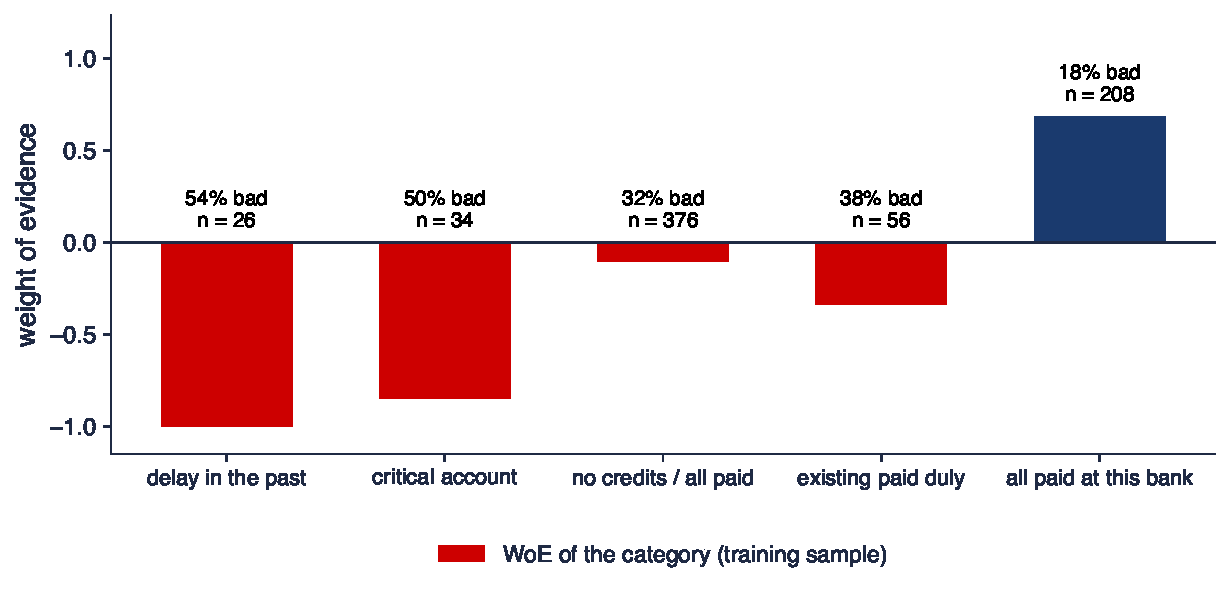
\includegraphics[width=0.96\textwidth,height=0.32\textheight,keepaspectratio]{ch12_sem_b1.pdf}
\end{center}
\vspace{-2mm}
\begin{center}
\tiny
\begin{tabular}{lrrrrrrr}
\toprule
& termen liber & contul curent & istoricul de credit & destinația creditului & economiile & durata & vechimea la angajator \\
\midrule
IV & & $0{,}591$ & $0{,}215$ & $0{,}205$ & $0{,}166$ & $0{,}159$ & $0{,}122$ \\
$\hat\beta$ & $-0{,}850$ & $-0{,}829$ & $-0{,}675$ & $-0{,}937$ & $-0{,}726$ & $-1{,}082$ & $-0{,}873$ \\
se & $0{,}095$ & $0{,}127$ & $0{,}206$ & $0{,}217$ & $0{,}246$ & $0{,}239$ & $0{,}265$ \\
\bottomrule
\end{tabular}
\end{center}
\begin{itemize}
    \item 6 variabile cu IV $\ge 0{,}1$; AUC: estimare $0{,}789$, test $0{,}801$, CI 95\% $[0{,}749; 0{,}854]$
    \item Interpretare: da: o întîrziere în trecut (54\% neperformante) și un cont critic (50\%) sînt cele mai riscante, toate creditele la această bancă rambursate la timp (18\%) cele mai sigure; în etichetele UCI necorectate, acest grup, cel mai sigur, se numea „cont critic”
\end{itemize}\sfmquantlet{Ch_12}{SFM_ch12_seminar}
\end{frame}

\begin{frame}{B2: Information Value pentru datele din Taiwan [Propus]}
\itemsize{\footnotesize}
\begin{itemize}
\item \textbf{Întrebarea}: ce fel de informație prezice nerambursarea unui deținător de card: comportamentul de plată sau datele personale? Model: B1.
\item \textbf{Date}: cardurile de credit din Taiwan, 30\,000 de clienți; aceeași împărțire stratificată 70/30
\item \textbf{Cerințe}
\begin{enumerate}
    \item Calculați IV pentru \texttt{PAY\_0} și \texttt{PAY\_2} (starea plăților în septembrie și august; categoriile de la $-2$ la 3 sau mai mult), pentru \texttt{LIMIT\_BAL}, \texttt{PAY\_AMT1}, \texttt{BILL\_AMT1} și \texttt{AGE} (quintile) și pentru \texttt{SEX}, \texttt{EDUCATION} și \texttt{MARRIAGE} (categorii) pe eșantionul de estimare.
    \item Calculați rata de nerambursare pentru fiecare categorie \texttt{PAY\_0}.
    \item Ordonați variabilele după IV și clasificați-le cu regula practică.
    \item Interpretare: de ce este starea plății din ultima lună mult mai puternică decît datele personale?
\end{enumerate}
\item \textbf{Raportați}: un tabel cu nouă valori IV, șase rate de nerambursare și două fraze
\item Notebook: secțiunea B2
\end{itemize}
\end{frame}

\ifsolutions
\begin{frame}{B2: rezolvare [Propus]}
\itemsize{\footnotesize}
\begin{center}
\scriptsize
\begin{tabular}{lrrrrrrrrr}
\toprule
& \texttt{PAY\_0} & \texttt{PAY\_2} & \texttt{LIMIT} & \texttt{PAY\_AMT1} & \texttt{EDUC.} & \texttt{AGE} & \texttt{MARR.} & \texttt{BILL\_AMT1} & \texttt{SEX} \\
\midrule
IV & $0{,}869$ & $0{,}564$ & $0{,}157$ & $0{,}148$ & $0{,}036$ & $0{,}013$ & $0{,}009$ & $0{,}009$ & $0{,}007$ \\
\bottomrule
\end{tabular}
\end{center}
\begin{itemize}
    \item Rata de nerambursare după \texttt{PAY\_0}: $-2$: 13{,}3\%; $-1$: 16{,}9\%; 0: 12{,}9\%; 1: 33{,}1\%; 2: 69{,}0\%; 3 sau mai mult: 73{,}4\%
    \item \texttt{PAY\_0} și \texttt{PAY\_2}: puternice; limita și plata: medii; educația: slabă; vîrsta, starea civilă, factura și sexul: inutile
    \item Interpretare: un client care întîrzie deja două luni a parcurs mare parte din drumul spre nerambursare: comportamentul măsoară rezultatul aproape direct, datele personale doar prin medii
\end{itemize}\sfmquantlet{Ch_12}{SFM_ch12_seminar}
\end{frame}
\fi

\begin{frame}{B3: validarea scorecard-ului [Rezolvat]}
\itemsize{\footnotesize}
\begin{itemize}
\item \textbf{Întrebarea}: cît de bun este scorecard-ul din B1 pe eșantionul de test și ce prag ar trebui să folosească banca?
\item \textbf{Date}: cele 300 de credite de test din B1 cu PD-urile lor; costuri: 5 pentru un rău-platnic acceptat, 1 pentru un bun-platnic respins
\item \textbf{Cerințe}
\begin{enumerate}
    \item Construiți matricea de confuzie la pragurile 0,5 și 1/6, cu acuratețea, TPR, FPR și costul pe solicitant.
    \item Calculați AUC, Gini, raportul de acuratețe al curbei CAP și statistica KS.
    \item Calculați scorul Brier, comparați-l cu o PD constantă de 30\% și aplicați testul Hosmer--Lemeshow cu cinci grupuri.
    \item Reprezentați curba ROC cu cele două praguri și graficul de calibrare.
    \item Interpretare: ce prag i-ați recomanda băncii?
\end{enumerate}
\item \textbf{Raportați}: un tabel cu două matrice de confuzie, șase statistici, graficul și două fraze
\item Notebook: secțiunea B3
\end{itemize}
\end{frame}

\begin{frame}{B3: rezolvare [Rezolvat]}
\itemsize{\scriptsize}
\begin{center}
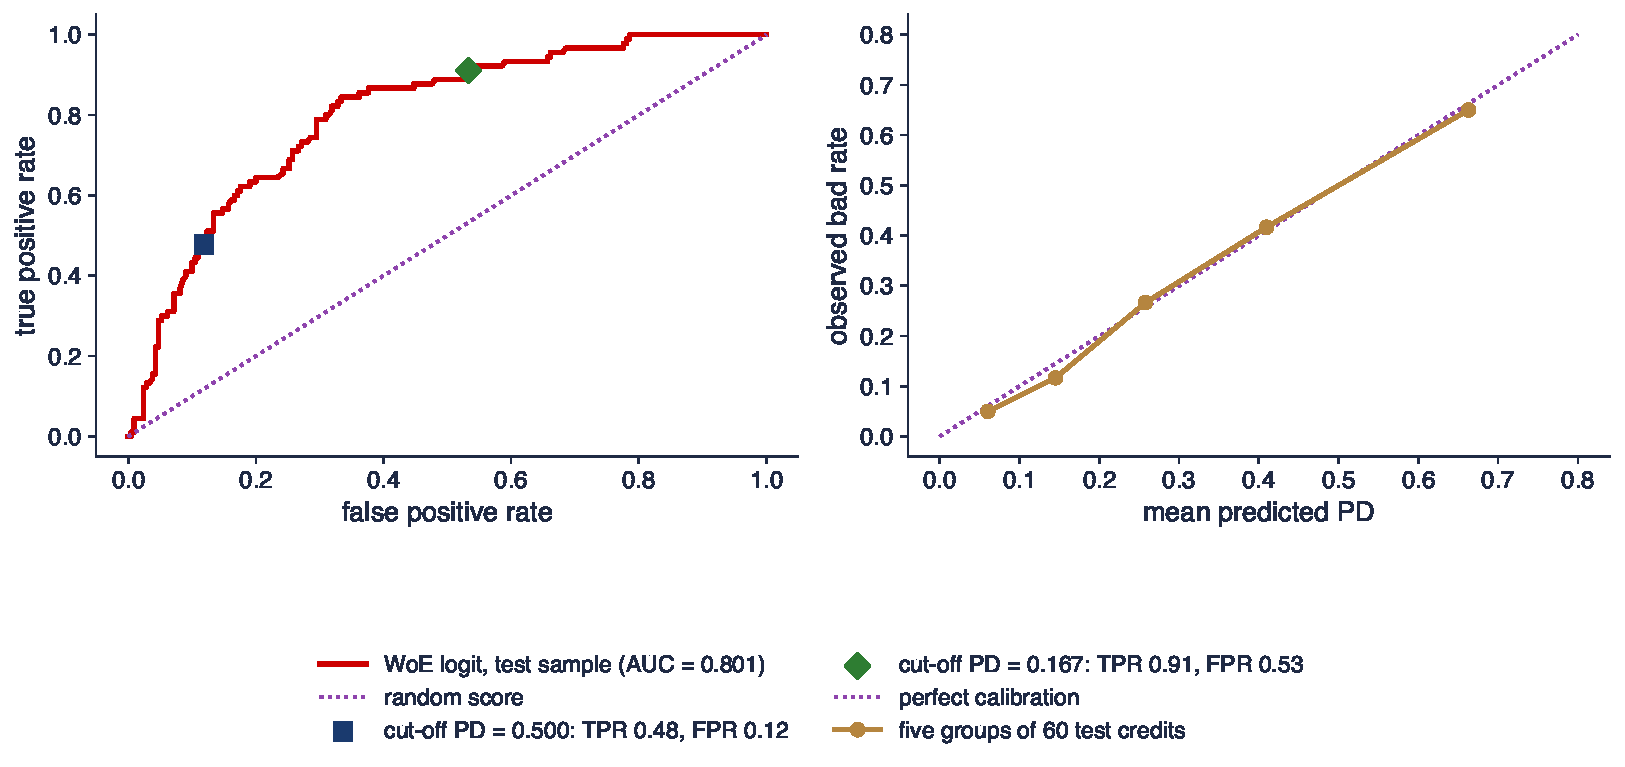
\includegraphics[width=0.96\textwidth,height=0.30\textheight,keepaspectratio]{ch12_sem_b3.pdf}
\end{center}
\vspace{-2mm}
\begin{center}
\tiny
\begin{tabular}{lrrrrrrrr}
\toprule
prag & TP & FN & FP & TN & acuratețe & TPR & FPR & cost \\
\midrule
0.5 & 43 & 47 & 25 & 185 & $76{,}0\%$ & $47{,}8\%$ & $11{,}9\%$ & $0{,}867$ \\
1/6 & 82 & 8 & 112 & 98 & $60{,}0\%$ & $91{,}1\%$ & $53{,}3\%$ & $0{,}507$ \\
\bottomrule
\end{tabular}
\end{center}
\begin{itemize}
    \item AUC $= 0{,}801$, Gini $= 0{,}603$, AR $= 0{,}602$, KS $= 0{,}511$; Brier $= 0{,}162$ față de $0{,}210$; HL $= 0{,}589$ (p $= 0{,}899$): nicio dovadă de calibrare greșită
    \item Interpretare: pragul de 1/6: respinge mai mulți solicitanți (64{,}7\%), dar identifică 91{,}1\% din rău-platnici, iar costul scade de la 0{,}867 la 0{,}507; acuratețea este un criteriu greșit cînd erorile au costuri diferite
\end{itemize}\sfmquantlet{Ch_12}{SFM_ch12_seminar}
\end{frame}

\begin{frame}{B4: logit sau LDA pe datele din Taiwan? [Propus]}
\itemsize{\footnotesize}
\begin{itemize}
\item \textbf{Întrebarea}: diferă logit-ul și LDA a lui Fisher prin ordonare sau prin calibrare? Model: B3.
\item \textbf{Date}: Taiwan, împărțire 70/30; 13 variabile standardizate: logaritmul limitei, vîrsta, indicatorii stării plății din septembrie, numărul lunilor cu întîrziere, gradul de utilizare, logaritmul plăților
\item \textbf{Cerințe}
\begin{enumerate}
    \item Estimați un logit și o LDA pe eșantionul de estimare cu aceleași variabile.
    \item Calculați AUC de test pentru ambele și testul DeLong de egalitate a AUC.
    \item Calculați scorul Brier, statistica Hosmer--Lemeshow (zece grupuri) și PD medie pentru ambele, față de rata de nerambursare.
    \item Calculați acuratețea regulii „nimeni nu intră în nerambursare” și a celor două modele la pragul 0,5.
    \item Interpretare: este LDA mai slabă la ordonare sau la calibrare?
\end{enumerate}
\item \textbf{Raportați}: un tabel și două fraze
\item Notebook: secțiunea B4
\end{itemize}
\end{frame}

\ifsolutions
\begin{frame}{B4: rezolvare [Propus]}
\itemsize{\footnotesize}
\begin{center}
\scriptsize
\begin{tabular}{lrrrrrr}
\toprule
& AUC & Brier & HL & PD medie & acuratețe (0,5) & TPR (0,5) \\
\midrule
logit & $0{,}777$ & $0{,}136$ & $40{,}7$ & $21{,}9\%$ & $81{,}9\%$ & $33{,}6\%$ \\
LDA & $0{,}778$ & $0{,}139$ & $282{,}5$ & $20{,}0\%$ & $81{,}9\%$ & $36{,}8\%$ \\
\bottomrule
\end{tabular}
\end{center}
\begin{itemize}
    \item DeLong: $z = -1{,}80$, p $= 0{,}072$; corelația logaritmilor șansei $0{,}993$; rata de nerambursare în test 22{,}1\%; „nimeni nu intră în nerambursare”: acuratețe 77{,}9\%
    \item Ambele modele depășesc regula trivială cu doar 4{,}0 puncte procentuale de acuratețe, dar identifică aproximativ o treime din nerambursări
    \item Interpretare: la calibrare: ordonarea este aceeași (AUC egale la 5\%), dar PD-urile LDA sînt deplasate (HL 282{,}5 față de 40{,}7), deoarece variabilele sînt indicatori și asimetrice, departe de distribuția Normală
\end{itemize}\sfmquantlet{Ch_12}{SFM_ch12_seminar}
\end{frame}
\fi

\begin{frame}{B5: de la PD la capital [Rezolvat]}
\itemsize{\footnotesize}
\begin{itemize}
\item \textbf{Întrebarea}: cîtă pierdere așteptată și cît capital Basel are portofoliul de test din B1 și cît contează corecția a priori?
\item \textbf{Date}: cele 300 de credite de test din B1; EAD $=$ suma creditului; LGD $= 45\%$; rata din populație 5\%; alte expuneri de retail
\item \textbf{Cerințe}
\begin{enumerate}
    \item Corectați PD a fiecărui credit de la rata de 30\% din eșantion la rata de 5\% din populație.
    \item Calculați pierderea așteptată a portofoliului, în DM și ca pondere din EAD, cu și fără corecție.
    \item Calculați capitalul IRB $K$ și activele ponderate la risc ale portofoliului cu PD corectate.
    \item Interpretare: de ce schimbă corecția pierderea așteptată, dar nu și AUC?
\end{enumerate}
\item \textbf{Raportați}: opt valori și două fraze
\item Notebook: secțiunea B5
\end{itemize}
\end{frame}

\begin{frame}{B5: rezolvare [Rezolvat]}
\itemsize{\footnotesize}
\begin{itemize}
    \item Corecția logaritmului șansei: $\ln(0{,}05/0{,}95) - \ln(0{,}30/0{,}70) = -2{,}097$
    \begin{itemize}
        \item PD medie: 30{,}7\% pe scala eșantionului, 7{,}3\% după corecție (mediana 4{,}2\%, maximul 54{,}4\%)
    \end{itemize}
    \item EAD 957\,819 DM; EL 41\,744 DM $=$ 4{,}4\% din EAD (fără corecție: 16{,}3\%)
    \begin{itemize}
        \item capitalul IRB $K$: 54\,542 DM $=$ 5{,}7\% din EAD; RWA 681\,771 DM, o pondere de risc de 71{,}2\%
    \end{itemize}
    \item PD medie corectată este peste 5\%, deoarece corecția se aplică logaritmului șansei, nu PD
    \item Interpretare: corecția adaugă aceeași constantă la fiecare logaritm al șansei: ordinea solicitanților, deci AUC, nu se schimbă, în timp ce fiecare PD scade, iar EL coboară de la 16{,}3\% la 4{,}4\% din EAD
\end{itemize}\sfmquantlet{Ch_12}{SFM_ch12_seminar}
\end{frame}

\begin{frame}{B6: echitatea pe datele din Taiwan [Propus]}
\itemsize{\footnotesize}
\begin{itemize}
\item \textbf{Întrebarea}: tratează logit-ul din B4 în mod egal bărbații și femeile, precum și clienții tineri și pe cei mai în vîrstă? Model: B5 și slide-ul 5/5.
\item \textbf{Date}: eșantionul de test din Taiwan (9000 de clienți); sexul și vîrsta nu sînt variabile ale modelului; aprobăm cei 75\% cu PD cea mai mică
\item \textbf{Cerințe}
\begin{enumerate}
    \item Calculați rata de aprobare și rata de nerambursare pentru bărbați și femei, precum și pentru clienții de pînă la 25 de ani și cei mai în vîrstă.
    \item Calculați rata de aprobare a bun-platnicilor (egalitatea de șanse) în fiecare grup.
    \item Calculați rata de nerambursare printre clienții aprobați din fiecare grup.
    \item Interpretare: de care criteriu de echitate se apropie cel mai mult modelul?
\end{enumerate}
\item \textbf{Raportați}: un tabel și două fraze
\item Notebook: secțiunea B6
\end{itemize}
\end{frame}

\ifsolutions
\begin{frame}{B6: rezolvare [Propus]}
\itemsize{\footnotesize}
\begin{center}
\scriptsize
\begin{tabular}{lrrrrr}
\toprule
& $n$ & rata de nerambursare & aprobați & bun-platnici aprobați & rău-platnici printre aprobați \\
\midrule
bărbați & 3\,574 & $24{,}7\%$ & $72{,}5\%$ & $83{,}2\%$ & $13{,}6\%$ \\
femei & 5\,426 & $20{,}5\%$ & $76{,}6\%$ & $85{,}1\%$ & $11{,}6\%$ \\
vîrsta $\le$ 25 & 1\,153 & $25{,}8\%$ & $68{,}3\%$ & $80{,}0\%$ & $13{,}1\%$ \\
vîrsta $>$ 25 & 7\,847 & $21{,}6\%$ & $76{,}0\%$ & $85{,}0\%$ & $12{,}3\%$ \\
\bottomrule
\end{tabular}
\end{center}
\begin{itemize}
    \item Pragul PD $= 23{,}5\%$; diferențe femei $-$ bărbați: aprobare $4{,}1$ puncte procentuale, bun-platnici $2{,}0$; peste 25 de ani $-$ pînă la 25 de ani: $7{,}6$ și $5{,}0$ puncte procentuale
    \item Interpretare: egalitatea de șanse: diferențele dintre bun-platnici (2{,}0 și 5{,}0 puncte procentuale) sînt mai mici decît diferențele de aprobare (4{,}1 și 7{,}6), care reflectă mai ales ratele diferite de nerambursare; paritatea ar cere praguri diferite pe grupuri
\end{itemize}\sfmquantlet{Ch_12}{SFM_ch12_seminar}
\end{frame}
\fi


%=============================================================================
\section{Partea C: întrebări deschise și critica unui răspuns AI}
%=============================================================================

\begin{frame}{C1: învinge gradient boosting logit-ul? [Propus]}
\itemsize{\footnotesize}
\begin{itemize}
\item \textbf{Întrebarea}: comparațiile raportează cîștiguri pentru modelele flexibile \refLessmann; cît de mare este cîștigul pe datele din Taiwan și merită pierderea unui scorecard simplu?
\item \textbf{Date}: variabilele și împărțirea din B4; modele: B3, B4
\item \textbf{Cerințe}
\begin{enumerate}
    \item Estimați gradient boosting (scikit-learn, setările implicite) pe eșantionul de estimare.
    \item Comparați AUC de test cu cel al logit-ului prin testul DeLong și comparați scorurile Brier.
    \item Comparați AUC de estimare și de test pentru gradient boosting.
    \item Interpretare: este cîștigul suficient de mare pentru a înlocui scorecard-ul?
\end{enumerate}
\item \textbf{Raportați}: un tabel și un plan de proiect
\item Notebook: secțiunea C1
\end{itemize}
\end{frame}

\ifsolutions
\begin{frame}{C1: analiză de referință [Propus]}
\itemsize{\footnotesize}
\begin{center}
\scriptsize
\begin{tabular}{lrrr}
\toprule
& AUC de test & Brier & AUC de estimare \\
\midrule
gradient boosting & $0{,}784$ & $0{,}134$ & $0{,}827$ \\
logit & $0{,}777$ & $0{,}136$ & $0{,}777$ \\
\bottomrule
\end{tabular}
\end{center}
\begin{itemize}
    \item DeLong: $z = 2{,}61$, p $= 0{,}009$: un cîștig semnificativ, dar mic (sub 0,01 în AUC); boosting-ul supraajustează și mai mult (AUC de estimare 0{,}827)
    \item Designul proiectului: validare încrucișată repetată, măsuri de cost și de echitate pe grupuri, explicații pentru modelul boosting și valoarea în bani a cîștigului (Lessmann et al.)
\end{itemize}\sfmquantlet{Ch_12}{SFM_ch12_seminar}
\end{frame}
\fi

\begin{frame}{C2: verificați un răspuns AI [Propus]}
\itemsize{\scriptsize}
\begin{itemize}
    \item Un student a cerut unui asistent AI să rezume scorecard-ul din B1. Răspunsul:
    \item \aiprompt{(a) AUC este 0{,}80, deci scorecard-ul clasifică corect 0{,}80 din solicitanți.}
    \item \aiprompt{(b) Coeficientul Gini este AUC - 0,5 = 0{,}30.}
    \item \aiprompt{(c) Un solicitant cu PD de 30\% din acest model are o probabilitate de 30\% de nerambursare la bancă.}
    \item \aiprompt{(d) Cu PDO = 20, o PD care scade la jumătate, de la 20\% la 10\%, adaugă exact 20 de puncte.}
    \item \aiprompt{(e) KS este cea mai mare distanță verticală dintre distribuțiile scorurilor rău-platnicilor și bun-platnicilor.}
    \item \aiprompt{(f) LDA poate fi folosită doar cînd fiecare variabilă are distribuția Normală.}
    \item Cerințe
    \begin{itemize}
        \item 1. Pentru fiecare afirmație, precizați dacă este corectă; dacă nu este, formulați afirmația corectă și, acolo unde se poate, dați valoarea corectă din notebook (secțiunea C2).
        \item 2. Raportați: o listă de șase verdicte, fiecare cu un rînd de justificare.
    \end{itemize}
\end{itemize}
\end{frame}

\ifsolutions
\begin{frame}{C2: rezolvare [Propus]}
\itemsize{\footnotesize}
\begin{itemize}
    \item (a) Greșit: AUC este probabilitatea ca un rău-platnic aleator să aibă o PD mai mare decît un bun-platnic aleator; acuratețea la 0,5 este 76{,}0\%
    \item (b) Greșit: Gini $= 2\,\mathrm{AUC} - 1 = 0{,}603$
    \item (c) Greșit: eșantionul are 30\% rău-platnici, banca aproximativ 5\%; după corecția a priori, PD este 5{,}0\%
    \item (d) Greșit: PDO dublează șansa bun:rău, nu PD: de la 4:1 la 9:1, scorul crește de la 527{,}1 la 550{,}5, adică 23{,}4 puncte
    \item (e) Corect: $\max_s|F_{\text{rău}}(s) - F_{\text{bun}}(s)|$
    \item (f) Greșit: criteriul Fisher nu cere nicio distribuție; normalitatea cu covarianță comună este necesară doar pentru PD a posteriori corecte (B4)
\end{itemize}\sfmquantlet{Ch_12}{SFM_ch12_seminar}
\end{frame}
\fi


%=============================================================================
\section{Încheiere}
%=============================================================================

\begin{frame}{Idei de reținut}
\itemsize{\small}
\begin{itemize}
    \item Un logit modelează logaritmul șansei; $e^{\beta}$ este un raport al șanselor; efectul asupra PD este $p(1 - p)\beta$
    \item WoE și IV transformă un tabel de bun-platnici și rău-platnici într-o dovadă și o ordonare a variabilelor
    \item AUC numără perechile ordonate corect; Gini $= 2\,$AUC $- 1$; acuratețea înșală cînd clasele sînt dezechilibrate
    \item Alegem pragul din costuri; corectăm PD din eșantioane suprareprezentate înaintea oricărui calcul de EL sau capital
    \item Un răspuns AI este o ciornă: verificați ce înseamnă AUC, formula Gini, corecția a priori și scala PDO
\end{itemize}
\end{frame}

\begin{frame}{După seminar}
\itemsize{\small}
\begin{itemize}
    \item Cursul 12 dezvoltă fiecare temă de azi: parametrii Basel, WoE și IV, logit și LDA, scorecard-urile, validarea, reject inference, echitatea, Altman și Merton
    \item Încercați cerințele [Propus] în notebook; rezolvările se discută la seminar
    \item C1 poate deveni un proiect de echipă: comparație prin validare încrucișată, costuri și echitate pe grupuri
    \item Lectură: \refFHH, cap.~21--22; \refMVA, cap.~14; \refSiddiqi
\end{itemize}
\end{frame}


%=============================================================================
\section{Bibliografie}
%=============================================================================

\begin{frame}{Bibliografie}
\itemsize{\tiny}
\begin{itemize}
    \item Basel Committee on Banking Supervision (2006). \href{https://www.bis.org/publ/bcbs128.htm}{International convergence of capital measurement and capital standards: a revised framework (comprehensive version)}. Bank for International Settlements.
    \item Brier, G.W. (1950). \href{https://doi.org/10.1175/1520-0493(1950)078<0001:VOFEIT>2.0.CO;2}{Verification of forecasts expressed in terms of probability}. \textit{Monthly Weather Review}, 78(1), 1--3.
    \item Cox, D.R. (1958). \href{https://doi.org/10.1111/j.2517-6161.1958.tb00292.x}{The regression analysis of binary sequences}. \textit{Journal of the Royal Statistical Society, Series B}, 20(2), 215--232.
    \item Default of Credit Card Clients [data set] (2009). \href{https://doi.org/10.24432/C55S3H}{UCI Machine Learning Repository}, CC BY 4.0.
    \item DeLong, E.R., DeLong, D.M., Clarke-Pearson, D.L. (1988). \href{https://doi.org/10.2307/2531595}{Comparing the areas under two or more correlated receiver operating characteristic curves: a nonparametric approach}. \textit{Biometrics}, 44(3), 837--845.
    \item Fisher, R.A. (1936). \href{https://doi.org/10.1111/j.1469-1809.1936.tb02137.x}{The use of multiple measurements in taxonomic problems}. \textit{Annals of Eugenics}, 7(2), 179--188.
    \item Franke, J., Härdle, W.K., Hafner, C.M. (2019). \href{https://doi.org/10.1007/978-3-030-13751-9}{\textit{Statistics of Financial Markets: An Introduction}}, 5th ed. Springer.
    \item Grömping, U. (2019). \href{http://www1.beuth-hochschule.de/FB_II/reports/Report-2019-004.pdf}{South German credit data: correcting a widely used data set}. Reports in Mathematics, Physics and Chemistry 4/2019, Beuth University of Applied Sciences Berlin.
    \item Hanley, J.A., McNeil, B.J. (1982). \href{https://doi.org/10.1148/radiology.143.1.7063747}{The meaning and use of the area under a receiver operating characteristic (ROC) curve}. \textit{Radiology}, 143(1), 29--36.
    \item Härdle, W.K., Simar, L. (2019). \href{https://doi.org/10.1007/978-3-030-26006-4}{\textit{Applied Multivariate Statistical Analysis}}, 5th ed. Springer.
    \item Hardt, M., Price, E., Srebro, N. (2016). \href{https://arxiv.org/abs/1610.02413}{Equality of opportunity in supervised learning}. \textit{Advances in Neural Information Processing Systems} 29; arXiv:1610.02413.
    \item Hosmer, D.W., Lemeshow, S. (1980). \href{https://doi.org/10.1080/03610928008827941}{Goodness of fit tests for the multiple logistic regression model}. \textit{Communications in Statistics -- Theory and Methods}, 9(10), 1043--1069.
    \item Lessmann, S., Baesens, B., Seow, H.-V., Thomas, L.C. (2015). \href{https://doi.org/10.1016/j.ejor.2015.05.030}{Benchmarking state-of-the-art classification algorithms for credit scoring: an update of research}. \textit{European Journal of Operational Research}, 247(1), 124--136.
    \item Siddiqi, N. (2006). \href{https://doi.org/10.1002/9781119201731}{\textit{Credit Risk Scorecards: Developing and Implementing Intelligent Credit Scoring}}. Wiley.
    \item South German Credit [data set] (2020). \href{https://doi.org/10.24432/C5QG88}{UCI Machine Learning Repository}, CC BY 4.0.
\end{itemize}
\end{frame}

\end{document}
